    % It has been impossible to complete this work without reflecting on the immense, indecent privilege of being able to do so. In a time of such great global turmoil, marked by the horrors of the war in Ukraine and the genocides in the Congo, Sudan, and Gaza, dedicating years to abstract problems can feel like a luxury that is difficult to justify.
    % What has kept me going is the idea that pushing forward the boundaries of knowledge is a fundamentally hopeful act. It is a wager on a future where humanity's greatest challenges are intellectual, not self-inflicted. It is a commitment to building rather than breaking. For their part in sustaining this small act of hope, and for keeping me grounded throughout this journey, I owe my deepest thanks to...

\chapter{Introduction}
\label{chap:introduction}
This thesis addresses some theoretical and algorithmic questions in computational physics from the mathematical point of view. More specifically, our contributions are motivated by persistent difficulties in the measurement of dynamical properties of molecular systems, both in the equilibrium and nonequilibrium setting, using stochastic models of the molecular dynamics (MD).
Before going into further detail regarding these contributions, we introduce in Section~\ref{sec:01:MD} the general context of MD simulations, discussing some historical aspects of the field's development, as well as the necessary theory to understand the mathematical aspects of MD simulations, with a focus on the targeting of dynamical properties.
In so doing, we will find that the main obstruction to the sampling of informative trajectories is~\textit{metastability}, a phenomenon of central importance in this thesis. The main mathematical approaches to understand metastability and various associated numerical methods are reviewed in Section~\ref{sec:01:metastability}. We finally summarize our contributions in Section~\ref{sec:01:contributions}.

\section{An overview of molecular dynamics}
\label{sec:01:MD}
Molecular dynamics is a set of techniques aimed at extracting properties of atomistic systems from carefully designed computer simulations. For details on the associated algorithms and additional background on MD from an applied perspective, we refer the interested reader to~\cite{AT17,FS01,T10}.
Due to the development of flexible and efficient methodologies, as well as the steady increase in available computational power over the last seventy years, MD has become a mainstay of computational physics, and is now routinely used in a variety of scientific applications from computational thermodynamics and material science to drug discovery and cell biology.
Fundamentally, MD simulates the time-evolution of systems at the atomic scale, by treating atoms as classical point particles, whose trajectories are governed by a defined set of dynamical laws. From the simulation and recording of these trajectories, several important scientific needs can be covered. Indeed, MD is simultaneously:
\begin{itemize}
\item \textit{A means to measure properties of matter}: MD provides numerical estimators for thermodynamic, structural and dynamical quantities that may be difficult or impossible to measure experimentally, due to extreme conditions or prohibitive costs. Typical outputs include radial distribution functions, free-energy differences, pressure and enthalpy, defect formation energies, reaction rates, and transport coefficients. With sufficiently long sampling, MD yields statistically converged values that can be used to parametrize coarser models. The computation of dynamical properties, and the associated need for long-time microscopic sampling, are a central motivation for Chapters~\ref{02:chap:semiclassic},~\ref{chap:shape_optimization} and~\ref{04:chap:norton}.
  \item \textit{A numerical microscope}: MD simulations allows to resolve molecular trajectories at a level of detail which is far beyond the reach of physical experiments. The analysis of MD trajectories can help to visualize reaction pathways, identify transition states, observe collective rearrangements (such as nucleation, defect propagation or protein folding), and extract mechanistic hypotheses that guide theoretical developments and experiments. These insights are especially valuable for understanding rare events and conformational changes, where a single trajectory can reveal the sequence of microscopic steps behind an observed macroscopic transition. MD simulations can be understood as \textit{in silico} experiments, which have become an important tool of modern materials and biological research.
  \item \textit{A benchmark for new methods}: due to its inherent flexibility, it is perhaps unsurprising that a major use case of MD is the development and testing of novel numerical and modelling tools for computational science at large, which in turn become useful for MD itself. New methods are validated on MD testbeds precisely because realistic atomistic models naturally combine the challenges of high dimensionality, nonlinearity and multiscale behavior.
  \item \textit{A hurdle for theory}: high-fidelity MD simulations have themselves become a source of ``ground truth'' data. Notably, long trajectories produced on bespoke hardware~\cite{SDDKLSYBBCal08} are routinely used to test biophysical hypotheses and to train data-driven models. At the same time, algorithms used in MD simulations expose some interesting mathematical questions which are still a fruitful area of research, some of which we address in this thesis.
\end{itemize}

\paragraph{Orders of magnitude}
{
Appreciating the vast discrepancies between the atomic, macroscopic and computational realms is key to understanding the scope of molecular dynamics simulations. It is therefore instructive to review some of the characteristic scales at play.

\noindent
\begin{minipage}[t]{0.48\textwidth}
\textbf{Atomistic scales}
\begin{itemize}
    \item Macroscopic amounts of matter are counted in moles of molecules, which are multiples of Avogadro's number~$N_{\mathrm{A}}=6.022\times 10^{23}$. A centilitre of liquid water at room temperature contains about~$0.56$ moles of molecules.
    \item Length is measured in units of {\AA ngstr\"oms}, ($1$~\AA$\,=10^{-10}\,\mathrm{m}$). For example, the Bohr radius of hydrogen is~$0.529$~\AA, while the helix of B-DNA has a diameter of~$20$~\AA.
    \item Time is measured in units of femtoseconds,($1$\,fs$=10^{-15}$\,s), which is also the typical timestep for MD simulations. The fastest molecular motions, such as the period of hydrogen bond stretching vibrational modes, span the order of~$10\,\mathrm{fs}$.
\end{itemize}
\end{minipage}\hfill
\begin{minipage}[t]{0.48\textwidth}
\textbf{Computational scales}
\begin{itemize}
  \item A 2018 projection~\cite{RGR18} estimates the size of the global ``datasphere'' (the total amount of digital information on Earth) to reach $175$~zettabytes by 2025, which corresponds to~$0.29\,N_{\mathrm{A}}$~bytes.
  \item Typical consumer machines provide on the order of~$10^{12}$~bytes of persistent storage capacity, whereas data centers and high-performance computing facilities operate at the~$10^{15}$--$10^{18}$ bytes scale.
  \item Consumer CPUs and GPUs deliver on the order of~$10^{9}$--$10^{12}$ floating-point operations by second (FLOPS), while modern exascale machines target sustained performance at around~$10^{18}$~FLOPS~\cite{Sc22}.
\end{itemize}
\end{minipage}
}
\newline\newline
\noindent   
This profound disparity between available computational resources and atomic scales implies that MD will fall short of fully resolving the microscopic trajectories of macroscopic systems (say, a second-long evolution of a millimeter-sized sample) for a foreseeable future.

The floating-point operation cost of advancing the simulation by a single timestep typically scales linearly with the number of atoms in the system: this fact imposes a hard limit on the~$(\text{length}\times\text{system size})$ of a feasible simulation given available computational resources at any fixed time.
Critically, it also reveals a present bottleneck for observing phenomena of scientific interest: with timesteps on the order of $1$fs, simulating a single~$\mu$s of a system's evolution requires executing on the order of a billion sequential steps. Yet, many important processes are known to unfold over timescales of milliseconds to seconds, or even longer.

Nevertheless, landmark MD simulations have consistently scaled up to larger numbers of atoms (and also to longer simulation times, but for rather different reasons). 
Scaling in the spatial domain (i.e. increasing the number of atoms in the system) can be achieved by exploiting a common property of molecular systems, namely the~\textit{locality} of interactions. This property allows to distribute the cost of advancing the simulation by one timestep, leveraging parallel computing architectures and domain decomposition algorithms.
This locality is the enabling principle which allow the linear scaling of the cost of MD simulations with system size. The link between locality and scalability is as ancient as MD itself, and underpins some of the earliest algorithmic innovations in the field, such as neighbor lists~\cite{V67}.

The situation is seemingly bleaker in the time domain. The sequential nature of a trajectory forbids distributing the computational cost of a single long simulation across parallel simulations of shorter segments. At first glance, the only way to extend the achievable computational timescales is by hardware-level or low-level software optimizations of the simulation procedure.
This challenge is known as the~\textit{timescale problem} of MD. While progress has been made using this brute-force approach, today still, for a typical solvated protein, a full day of computation on a high-performance GPU yields, at best, a few hundred ns of trajectory time~\cite{HD18}, and still much less for the large systems of interest to materials science.

To enable the simulation of long trajectories for relevant systems (without requiring access to highly specialized hardware) sophisticated algorithms have to be developed to go beyond sequential MD. A class of such methods are the so-called~\textit{accelerated MD} methods pioneered by Arthur Voter~\cite{V97,V98,SV00}, which play a crucial role in this thesis, and which will be discussed in further detail in Section~\ref{sec:01:dynamical_properties} below.
Similarly to the algorithms allowing to scale in space, these methods rely on an enabling property of many molecular systems, namely their~\textit{metastability}. Loosely speaking, a metastable system spends the majority of its time in long-lived, quasi-stationary states, punctuated by rare and abrupt transitions between them.
Metastable systems have become an object of study in their own right in mathematical physics, for which many mathematical results have been obtained, some of which we review in Section~\ref{sec:01:metastability}, derive in Chapter 2, and apply in Chapter 3.

\paragraph{Some historical milestones.}
\label{par:01:milestones}
Despite these challenges, full-atom ``brute-force'' MD simulations have been successfully applied to various problems. Here we list some simulations, notable for their historical importance and/or their novel magnitude, both in the spatial and time domain.
\begin{itemize}
    \item{\textit{1953}: Metropolis et al.~\cite{MRTT53} compute the equation of state for a hard-sphere model using a Monte Carlo method, spawning the field of computational statistical physics. This early work is followed in \textit{1957} by the first simulation~\cite{AWal57} of the molecular dynamics of a hard sphere model.}
    \item{\textit{1964}: Rahman~\cite{R64} measures properties of liquid argon using a MD simulation of interacting Lennard--Jones particles. Results are consistent with experimental measurements. This is followed in~\textit{1971} by the more challenging case of liquid water~\cite{RS71} by Rahman and Stillinger.}
    \item{\textit{1975}: Levitt and Warshel~\cite{LW75} simulate a protein folding using a coarse-grained energy minimization procedure.}
    \item{\textit{1988}: Levitt and Sharon~\cite{LS88} perform the first simulation of a protein in explicit water solvent, a~$0.2$\,nanosecond-long trajectory.}
    \item{\textit{1998}: Duan and Kollman~\cite{DK98} publish the first microsecond-long simulation of a fast-folding protein in explicit solvent, the villin headpiece, exposing the intricate mechanisms underlying protein folding.}
    \item{\textit{2002}: Abraham et al.~\cite{AWGDDDLRS02} carry out the first MD simulation involving more than a billion atoms, a short trajectory of a flawed FCC crystal undergoing ductile failure.}
    \item{\textit{2008}: Germann and Kadau~\cite{GK08} report the first MD simulation involving a trillion atoms, 40 timesteps of a Lennard--Jones crystal.}
    \item{\textit{2010}: Shaw et al.~\cite{SMLLPDEBJSSal10} perform the first millisecond-long simulation of a protein in explicit solvent, using a dedicated machine design~\cite{SDDKLSYBBCal08}, and at great financial cost.}
    \item{\textit{2017}: Perilla and Schulten~\cite{PS17} publish a full-atom simulation of the HIV-1 viral capsid in water (64 million atoms for~$1.2\,\mu$s).}
\end{itemize}

Long MD trajectories provide valuable insight into the thermodynamic and kinetic properties of molecular systems, by revealing their microscopic states and how they change in time.
The framework of statistical mechanics, which we now introduce, connects the microscopic state of a physical system to its macroscopic properties, and in so doing provides the basis for the measurement of physical properties from simulation data.

\subsection{Elements of statistical mechanics}
Statistical mechanics is the rigorous attempt to reconcile the microscopic point of view, in which a system's many microscopic degrees of freedom evolve according to fundamental physical laws, and the macroscopic point of view, according to which only a handful of variables are relevant to describe the system's state and evolution.
Here, we present the necessary formalism to treat the molecular systems of interest in MD. In particular, we restrict our scope to classical systems.
We note however that a similar Gibbsian formalism also exists for quantum systems (see~\cite{F72}) and has been more generally used to great effect in the study of a variety of disordered systems, such as spin glasses~\cite{EA75}, Hopfield networks~\cite{P84} and their quantum counterparts~\cite{RY96,RMGLM18}.

\paragraph{Microscopic states, their energy and classical dynamics.}
In this thesis, we consider systems of $N>0$ point particles, representing classical atomic nuclei.
The system's microscopic configuration, or \textit{microstate}, is described by the positions and momenta of each one of these nuclei. The microstate therefore corresponds to a point in \textit{phase space}, 
\begin{equation}
    \label{eq:01:phase_space}
    (q,p)\in \cE := \cX\times \cM,
\end{equation}
where~$\cX$ is a configurational domain, and for a configuration~$(q,p)\in\cE$, $q\in\cX$ is the position variable, and~$p\in \cM$ is the associated momentum variable in the momentum space~$\cM$.

To each microstate~$(q,p)\in\cE$, we associate its energy~$H(q,p)$. The function~$H$ is called the~\textit{Hamiltonian}. In most situations,~$\cM=\R^{3N}$, and the Hamiltonian takes the separable form
\begin{equation}
    \label{eq:01:hamiltonian}
    H(q,p) = V(q) + \frac12p^\top M^{-1}p,\qquad M = \begin{pmatrix}
    m_1 \I_3 & 0 & \dotsm & 0 \\
    0 & m_2 \I_3 & \dotsm & 0 \\
    \vdots & \ddots & \ddots & \vdots\\
    & \dotsm & 0 & m_N \I_3 
\end{pmatrix}
\end{equation}
where~$V:\cX\to\R$ is a potential energy function, the term~$\frac12p^\top M^{-1}p$ gives the kinetic energy, and~$M$ is a diagonal matrix encoding the atomic masses in the system, with~$m_i>0$ giving the mass of the~$i$-th particle for~$1\leq i\leq N$.

The classical equations of motion, as described by Newton's second law, can then be written compactly using the Hamiltonian~\eqref{eq:01:hamiltonian}. They are equivalently expressed by the following ordinary differential equation in~$\cE$:
\begin{equation}
    \label{eq:01:hamiltonian_dynamics}
    \frac{\d}{\d t}\,X_t = -J\nabla H(X_t),\qquad X_t = (q_t,p_t)\in \cE,
\end{equation}
where~$J$ is the~\textit{symplectic matrix}
\begin{equation}
    \label{eq:01:J}
    J=\begin{pmatrix}
        0&\I_{3N}\\-\I_{3N}&0
    \end{pmatrix}.
\end{equation}
In this form, the equation~\eqref{eq:01:hamiltonian_dynamics} is known as~\textit{Hamiltonian dynamics}, and its trajectories in phase space describe the time-evolution of an isolated system of classical particles.

\paragraph{On the choice of the interaction potential~$V$.}
The potential~$V$ is the crucial physical parameter, as it encodes the interactions between nuclei, and therefore their dynamics. Ideally, it is defined by the ground-state energy of the electronic Hamiltonian in the Born--Oppenheimer approximation~\cite{BO27}:
\begin{equation}
    \label{eq:01:schrodinger}
    V_{\mathrm{BO}}(q) = \inf\left\{\left\langle\psi, H(q) \psi\right\rangle_{\mathcal H_\cX}:\,\psi \in \mathcal H^1_{\cX,q},\,\|\psi\|_{\mathcal H_\cX}=1\right\},
\end{equation}
where~$\mathcal H_{\cX}$ and~$H(q)$ are respectively the Hilbert space of electronic wave functions and the Schr\"odinger operator associated with a given position of classical nuclei~$q\in\cX$, and~$\mathcal H^1_{\cX,q}\subset \mathcal H_{\cX}$ is the associated form domain.

For systems of interest in MD, the problem~\eqref{eq:01:schrodinger} is a very high-dimensional partial differential equation (PDE) eigenvalue problem, and therefore cannot be solved directly. Instead, one resorts to a variety of approximations to estimate~$V_{\mathrm{BO}}$, or rather its gradient~$\nabla V_{\mathrm{BO}}$ with respect to~$q$; since the dynamics~\eqref{eq:01:hamiltonian_dynamics} only depends on the force~$\nabla V$, these classes of approximations are also known as~\textit{force fields}, of which we distinguish three main families.
\begin{itemize}
    \item{\textit{Ab initio methods} leverage the considerable work in electronic structure theory over the last 100 years. Many numerical methods have been developed to address the problem~\eqref{eq:01:schrodinger}: with no claim of exhaustivity, popular schemes include the Hartree--Fock method, the more precise (and costly) post--Hartree--Fock methods, as well as methods rooted in density functional theory (DFT), see~\cite{J99} for a comprehensive introduction. While such methods can be very accurate, as they incorporate quantum effects of the electronic structure in the classical nuclear dynamics, their poor scaling with respect to system size and their high cost of evaluation limit their applications to small systems and short simulation times. They are nevertheless essential to capture some phenomena, such as bond-breaking in chemical reactions.}
    \item{\textit{Empirical force fields}, which constitute the most important class of methods historically, proceed by first selecting a set of prototypical systems~$\mathcal S$, and for each~$s\in\mathcal S$, introducing a parametric ansatz~$V^{s}_\theta(q)$ for the minimum~\eqref{eq:01:schrodinger}. The functional form of~$V^s_\theta$ is hand-crafted to find a balance between physical principles and computational efficiency. To allow the functional form to be transferable to systems with varying number of atoms and molecular topologies,~$V^s_\theta$ is usually expressed as a sum of local energy contributions from each atom in~$s$, which are themselves functions of the corresponding~\textit{atomic environment}, given by the relative positions of neighboring atoms, their species, and their adjacency relationship in the covalent bond structure. A regression can then be performed to select an optimal parameter~$\theta^*$, in order to replicate a set of targeted thermodynamic or structural properties over~$\mathcal S$, measured either experimentally or using ab initio computations. The empirical potential~$V_{\theta^*}^{s'}$ can then be used to probe the system~$s'\not\in\mathcal S$.
    The oldest and simplest example of empirical potential is the Lennard--Jones pair-potential~(Equation~\eqref{eq:01:lennard_jones} below), which only uses two parameters, but many families of force-fields of this type are still widely used, such as CHARMM~\cite{BBOSSK83},~AMBER~\cite{PCCRCDFSK95} and GROMOS~\cite{SHTMBFTHKVG99} for biomolecules, EAM~\cite{DB84} for metallic systems, or Tersoff-type potentials~\cite{T89} for multi-species solids.}
    \item{\textit{Machine-learned interatomic potentials} (MLIPs) can be understood as the application of modern machine-learning architectures in the empirical approach described above. While they are conceptually the same, the two approaches nevertheless differ in that the parameter~$\theta$ no longer has any clear physical meaning. MLIPs has recently gathered interest, due to the hope of nearly matching the accuracy of ab-initio methods at a fraction of their computational cost. This promise has gained some credence in recent years, due to the demonstrated flexibility of various machine-learning architectures, and to the rapid increase in the availability of ab-initio training data. This class of models typically define the potential in two steps, by first computing for each atom a feature vector of so-called~\textit{descriptors} encoding its atomic environment, and designed to enforce some physical priors, such as the locality of interactions and various symmetries. Common choices include radial symmetry functions~\cite{BP07}, SOAP~\cite{BKC13} and ACE~\cite{D19} descriptors.
    In a second step, the descriptor is used as input to a machine-learning model, typically a linear model~\cite{TSTFT15}, neural network~\cite{BP07} or Gaussian process~\cite{BPKC10}, giving the energy contribution for a single atom. Summing over atoms gives the final functional form. Crucially, forces on each atom, which are required for dynamics (and training the model), can usually be computed efficiently using reverse-mode automatic differentiation~\cite{BPRS18}.
    }
\end{itemize}

To give a concrete example--which will be used in Chapter 3-- we consider the simplest variant of the AMBER~\cite{PCCRCDFSK95} force-field. It decomposes the potential energy into contributions associated with bond stretching, bond bending, torsional energy, and pairwise interactions, modelling Van der Waals and electrostatic interactions between nuclei.
More precisely,~$V(q)=\sum_{i=1}^{N}V_i(q)$, where for each atom~$1\leq i\leq N$, the local contribution~$V_i$ writes
\begin{equation}
\begin{split}
    \label{eq:01:amber}
    V_i(q)&=\sum_{\text{bonds}\,\{i,j\}} \frac{k_b^{ij}}{2}(r_{ij}-r_0^{ij})^2 + \sum_{\text{angles}\,\{i,j,k\}} \frac{k_a^{ij}}{2}(\alpha_{ijk}-\alpha_0^{ijk})^2 \\
    &+ \sum_{\text{dihedrals}\,\{i,j,k,\ell\}} E^{ijk\ell}\left(1+\cos(n^{ijk\ell}\phi_{ijk\ell}-\gamma^{ijk\ell})\right) \\
    &+ \frac12\sum_{j\neq i}\left(4\varepsilon_{ij}\left[\left(\frac{\sigma^{ij}}{r_{ij}}\right)^{12}-\left(\frac{\sigma^{ij}}{r_{ij}}\right)^6\right] + \frac{C^{ij}}{r_{ij}}\right),
\end{split}
\end{equation}
where the first three sums give the so-called~\textit{bonded} energy contributions, and run over covalent bond chains of increasing length involving atom~$i$: 2-chains defining a bond length~$r_{ij}=|q_i-q_j|$, 3-chains defining a bond angle~$\alpha_{ijk}$, and 4-chains defining a dihedral (or torsional) angle~$\phi_{ijk\ell}$. The final two sums give the~\textit{non-bonded} contributions, respectively a Lennard--Jones type term, and a Coulombic interaction term. The various parameters~$\theta^{ijk\ell}=\left(k_b^{ij},r_0^{ij},k_a^{ijk},\alpha_0^{ijk},E^{ijk\ell},n^{ijk\ell},\gamma^{ijk\ell},\varepsilon^{ij},\sigma^{ij},C^{ij}\right)$ are determined by the atomic species of atoms~$i,j,k$ and~$\ell$, as well as their ordering in the covalent chain for bonded interaction terms.

For simpler systems, such as monoatomic noble-gas fluids, this general form reduces to the Lennard--Jones potential
\begin{equation}
    \label{eq:01:lennard_jones}
    V(q) = \sum_{1\leq i < j \leq N} V_{\mathrm{LJ}}\left(|q_i-q_j|\right),\qquad V_{\mathrm{LJ}}(r) = 4\varepsilon \left[\left(\frac{\sigma}{r}\right)^{12}-\left(\frac{\sigma}{r}\right)^6\right],
\end{equation}
which now only depends on two parameters, an energy~$\varepsilon$ and a length~$\sigma$, and which we will use in Chapter 4. It is represented for reference in Figure~\ref{01:fig:lj}.
\noe{ajouter figure(s)}
\begin{figure}
    \centering
    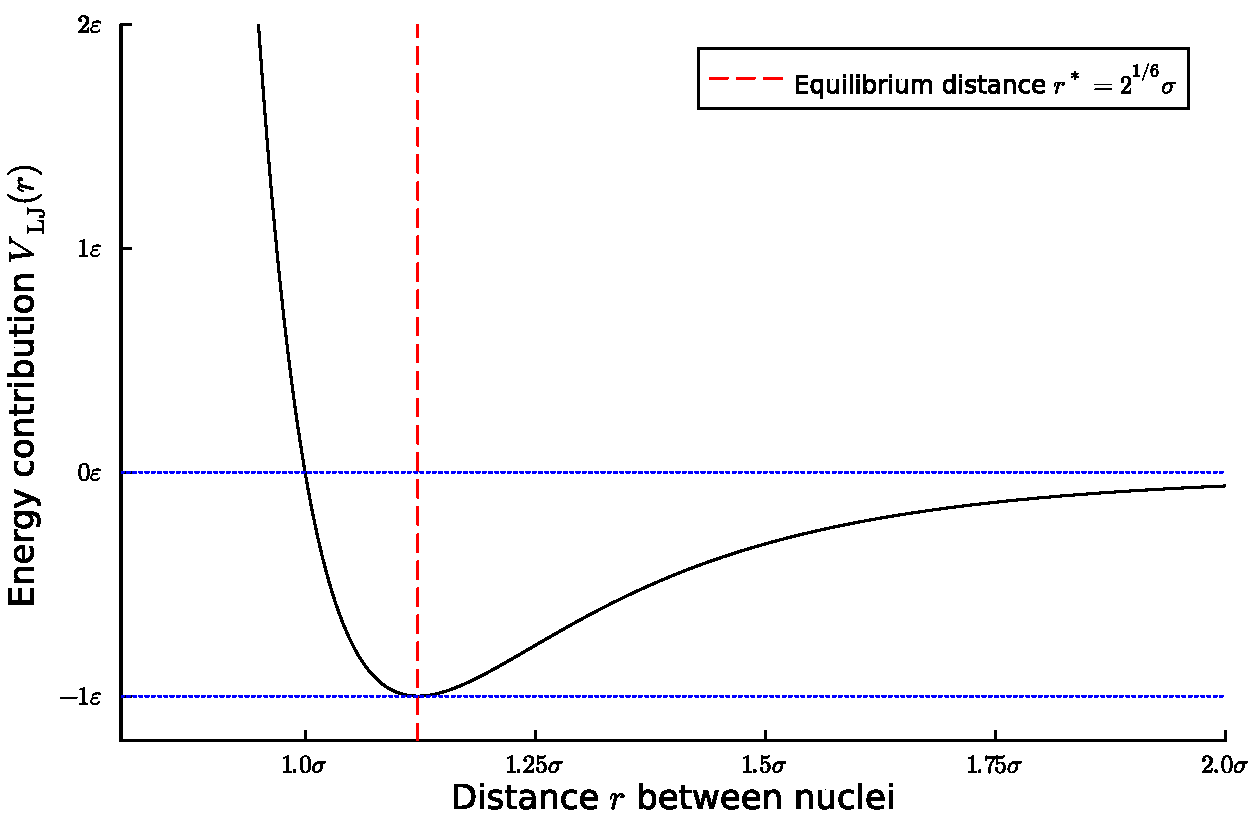
\includegraphics[width=0.8\textwidth]{figures/01/lj.pdf}
    \caption[The Lennard--Jones pairwise potential]{The pairwise Lennard--Jones potential defined in~\eqref{eq:01:lennard_jones}. The functional form imposes a Van der Waals-like attraction between nuclei further apart than the equilibrium distance~$r^*=2^{1/6}\sigma$, and a very strong repulsion between nuclei closer than~$r^*$.}
    \label{01:fig:lj}
\end{figure}

\paragraph{Boundary conditions.}
The specific definition of the phase space~$\cE$ depends on the physical model and properties of interest. We distinguish several common choices.
\begin{itemize}
    \item{\textit{Periodic boundary conditions}: this common choice corresponds to setting~$\cX = (L\T)^d$ and~$\cM=\R^d$, where~$\T=\R/\Z$ is the unit one-dimensional torus,~$d=3N$ is the number of position degrees of freedom in the system, and~$L>0$ is a length parameter fixing the size of the domain. This setup is essential for studying the bulk properties of matter, as the periodic unit cell models a small portion of the molecular medium while its images represent the surrounding environment, eliminating surface effects.}
    \item{\textit{Unbounded domains}: setting~$\cX$ and~$\cM$ equal to~$\R^d$ is appropriate for studying molecular systems in isolation, such as small atomic clusters or single molecules in vacuum.}
    \item{\textit{Non-flat position manifolds}: for certain applications, it is useful to restrict the particle positions to a non-flat manifold~$\cX$. This can be useful for enforcing geometric constraints, such as fixed bond length or angles, or for expressing the equations of motion in non-Cartesian coordinates~\cite{VJ15}. Such constraints can improve the stability of numerical schemes~\cite{RCB77,A83,BKLS95}, allowing for larger time steps, and can be used for computing free energy differences~\cite{SC98,LRS12}. In this geometric setting, the momentum associated to a given position~$q\in\cX$ is a cotangent vector~$p\in T_q^*\cX$, and the phase space~$\cE$ is the cotangent bundle:~$\cE=T^*\cX$, which no longer has the simple product form~\eqref{eq:01:phase_space}.}
    \item{\textit{Exotic boundary conditions}: for the purpose of some specialized simulations, one can consider a variety of additional boundary conditions. For instance, one can consider walls at the boundary of a domain~$\partial\cX$, on which particles are subject to specular or diffuse reflections, or absorption~(the role of absorbing boundaries is crucial in Chapters~2 and~3 of this thesis). Mixed conditions, which are periodic with respect to a subset of coordinates, can be used to study interfaces. One can even consider time-dependent definitions, such as Lees--Edwards boundary conditions~\cite{LE72}, which allow to study shear flows.}
\end{itemize}    
The choice of boundary conditions fixes the geometry of the phase space, the next step is to relate this collection of microstates to the macroscopic state of the system. 

\paragraph{Statistical ensembles.}
The basic postulate of statistical mechanics, as formalized by Gibbs in~\cite{G02}, is that the system's macroscopic configuration is a probability distribution~${\pi\in\cP(\cE)}$ over the set of possible microstates.
The distribution~$\pi$ is also known as a statistical or~\textit{thermodynamic ensemble}. In this statistical description, the ensemble~$\pi$ assigns to each microstate the likelihood of underlying the observed macrostate, and is therefore a crucial model parameter.

Given a physical observable~$\varphi:\cE\to\R$, we can then define the macroscopic value of~$\varphi$ as the~\textit{ensemble average}:
\begin{equation}
    \label{eq:01:ensemble_average}
    \langle \varphi\rangle_{\pi} = \E_\pi\left[\varphi\right]= \int_{\cE}\varphi\,\d \pi.
\end{equation}

For example, the pressure~$P$ of an isotropic fluid in a periodic box can be expressed as an ensemble average~\eqref{eq:01:ensemble_average} of the instantaneous bulk pressure:
\begin{equation}
    \label{eq:01:pressure}
    \varphi_P(q,p) = \frac{1}{3L^3}\left(p^\top M^{-1}p-q^\top\nabla V(q)\right),\qquad\text{where } V(q) = \sum_{1\leq i<j\leq N} w(|q_i-q_j|),
\end{equation}
and~$w:\R^+\to\R$ is a pairwise potential profile (such as the Lennard--Jones potential~$V_{\mathrm{LJ}}$ from Equation~\eqref{eq:01:lennard_jones}).

To make the definition operational, one should have a principled way to assign a specific ensemble to a given set of physical conditions.
We distinguish two families of methods to achieve this.

\begin{itemize}
    \item{\textit{Dynamical definitions}. In these constructions, the ensemble~$\pi$ is identified with an invariant probability measure or~\textit{steady state} of the system's underlying dynamics.
    Whether the dynamics are deterministic or stochastic, whenever the system is ergodic with respect to~$\pi$, time averages of observables along a single, long trajectory will converge to the ensemble average~\eqref{eq:01:ensemble_average}.
    This approach provides a physical justification for the ensemble by connecting it directly to the microscopic time-evolution of the system, in the case a model of the microscopic dynamics is available.
    It also the viewpoint which underpins theoretically the computation of macroscopic properties using equilibrium and nonequilibrium molecular dynamics.
    }
    \item{Variational definitions based on the \textit{principle of maximal entropy}, as described in \cite{J57a,J57b}, offer a fairly general alternative.
    This approach frames the problem of determining the ensemble from the knowledge of macroscopic data as one of statistical inference.
    Namely, the ensemble~$\pi$ is defined as the probability distribution which maximizes the information entropy, given by the ensemble average $S[\pi] = -\langle\log\pi\rangle_\pi$ (with some abuse of notation), subject to a set of constraints derived from the observation of the values of a number of macroscopic variables.
    Informally, this principle selects the most uninformative distribution compatible with the available information, and draws a connection between statistical mechanics and information theory. Solving for~$\pi$ generally leads to explicit expressions, independently of any hypotheses concerning the microscopic dynamics.}
\end{itemize}

\paragraph{Examples of statistical ensembles.}
We now give some examples, the first two of which were introduced by Gibbs in~\cite{G02}, and are of primary interest for MD.
\begin{itemize}
    \item{\textit{The microcanonical ensemble} ($NVE$) describes an isolated system with a fixed number of particles ($N$), volume ($V$), and total energy ($E$). It is given by the probability measure~$\pi_{NVE}$, where
    \begin{equation}
        \label{eq:01:microcanonical_distribution}
        \forall\,A\in\mathcal B(\cE),\qquad \pi_{NVE}(A) = \frac1{Z_{NVE}}\int_{A\cap H^{-1}(E)}|\nabla H|^{-1}\d\mathcal{H}_{H^{-1}(E)},
    \end{equation}
    where~$\mathcal{H}_{H^{-1}(E)}$ is the~$(d-1)$-dimensional Hausdorff measure on the constant-energy surface~$H^{-1}(E)$ and
    \[Z_{NVE}=\int_{H^{-1}(E)}|\nabla H|^{-1}\d\mathcal{H}_{H^{-1}(E)}\]
    is a normalizing constant known as the~\textit{microcanonical partition function}. Dynamically, it is the invariant measure of Hamiltonian dynamics~\eqref{eq:01:hamiltonian_dynamics} started at a point~$X_0\in H^{-1}(E)$, assuming the ergodic hypothesis.
    The choice of the microcanonical ensemble can also be motivated by postulating equiprobability for microstates of equal energy; the measure~$\pi_{NVE}$ can then be defined as the limit as~$\delta\to 0$ of uniform probability distributions on the energy shells~$\mathcal S(E,\delta):=H^{-1}(E-\delta,E+\delta)$, which are known to maximize the information entropy in~$\cP(\mathcal S(E,\delta))$ (whenever~$\mathcal S(E,\delta)$ is compact).}

    \item{\textit{The canonical ensemble} ($NVT$) describes a system with fixed number of particles and volume, in thermal equilibrium with a heat bath at a constant temperature $T$. It is given by the \textit{Boltzmann--Gibbs distribution}
    \begin{equation}
        \label{eq:01:boltzmann_gibbs}
        \forall\,A\in\mathcal B(\cE),\qquad \mu(A) = \frac{1}{Z_\mu(\beta)}\int_{A}\e^{-\beta H(q,p)}\,\d q\,\d p,
    \end{equation}
    where~$H$ is defined in~\eqref{eq:01:hamiltonian}, and~$\mu$ is parametrized by the parameter~$\beta = (k_{\mathrm{B}}T)^{-1}$, where~$k_{\mathrm{B}}$ is Boltzmann's constant and
    \[
    Z_\mu(\beta) = \int_{\cE}\e^{-\beta H(q,p)}\,\d q\,\d p
    \]
    is the~\textit{canonical partition function}.
    It correspond to invariant probability measure for a system evolving under various dynamics (often stochastic, some of which are discussed in Section~\ref{subsec:01:sampling} below) which model the interaction with the heat bath. From the point of view of the maximum entropy principle, it is derived by maximizing the information entropy subject to the constraint of a fixed \textit{average} energy, which is related to the temperature $T$ by the formula~${\langle H\rangle_{\mu} = -\frac{\partial}{\partial\beta}\log\,Z_\mu(\beta)}$. }
    \item{Other equilibrium ensembles can be constructed to model more general physical conditions. The \textit{isothermal-isobaric ensemble} ($NPT$) describes systems at constant temperature and pressure~$P$, which are sometimes relevant for biological applications, and is derived from the maximal entropy principle by fixing the average energy and average volume of the system (related to the pressure~$P$). The \textit{grand-canonical ensemble} ($\mu$VT) describes systems that can exchange both heat and particles with a bath, and is defined by fixing the average energy and average particle number (related to the chemical potential $\mu$).}
    \item{\textit{Nonequilibrium ensembles}, describe systems driven away from thermal equilibrium by the application of non-conservative forces or thermal gradients. These systems are characterized by the presence of irreversible fluxes and entropy production. Most often, these ensembles are defined dynamically, as the invariant measure of some nonequilibrium process, in which case the ensemble is also known as a nonequilibrium steady-states~(NESS). The question of finding variational constructions for nonequilibrium ensembles has been investigated in the physical literature~(see~\cite{J80}), but does not appear to be fully settled at this time.}
\end{itemize}
Finally, let us mention that \textit{equivalence of ensembles} results allow to relate averages in one ensemble to averages in another. For instance, it has been shown that, for systems with short-range interactions, the~$NVE$ and~$NVT$ ensembles are equivalent (in several ways, and under technical conditions, see~\cite{T15} for a detailed discussion) in the thermodynamic limit~$N,V\to +\infty$ keeping the particle density~$\rho = N/V$ fixed.
In particular, so called~\textit{macrostate equivalence} results imply that, for intensive observables~$\varphi$, the canonical averages~$\langle\varphi\rangle_{NVT}$  and corresponding microcanonical averages $\langle \varphi\rangle_{NVE}$ converge to a common limit when~$N\to +\infty$, where~$T$ and~${E=Nu}$ are chosen so that the canonical specific energy~$\langle H/N\rangle_{NVT}$ converges to the microcanonical one~$u$.
Equivalence results for nonequilibrium ensembles is also a current topic of interest, see~\cite{CT13} for an example.

\paragraph{Collective variables and canonical free-energies.}
An important quantity associated with the canonical ensemble is its Helmholtz free-energy
\begin{equation}
    \label{eq:01:helmholtz}
    A(\beta)=-\frac{1}{\beta}\,\log\,Z_\mu(\beta),
\end{equation}
from which a variety of thermodynamic properties may be deduced as a function of the free parameter~$\beta$. For instance, a simple formal computation shows that the Helmholtz free-energy, information entropy~$S(\beta) := -\langle \log(\e^{-\beta H}/Z_\mu(\beta))\rangle_{\mu}$ and internal energy~$U(\beta):=\langle H\rangle_{\mu}$ are related by the famous identity
\begin{equation}
    A(\beta) = U(\beta) - \frac1\beta S(\beta).
\end{equation}

Often, one is led to describe the microstate of the system with a~\textit{collective variable} (CV), also known as an order parameter or reaction coordinate. For simplicity, we consider here a one-dimensional CV, which is a map~$\xi:\cE\to\R$ (the extension to multi-dimensional CVs is discussed in Section~\ref{03:sec:coarse_graining} of Chapter~\ref{chap:shape_optimization}).
Generally, the CV~$\xi$ is chosen to summarize one of the microstate's key structural features: the value of some interatomic distance or angle, a measure of similarity with respect a reference microstate, or a progress metric along a reference trajectory are all common examples of CVs.
They are in many ways indispensable to get an intuitive understanding of the microstate of a large molecular system. 
In turn, the CV induces a summary description of the ensemble itself, via the pushforward measure~$\xi_*\pi \in \mathcal P(\R)$, defined by~$\xi_*\pi(A) = \pi(\xi^{-1}(A))$ for any measurable subset~$A\subset\R$.

In the case of the canonical ensemble~$\pi = \mu$, and if~$\xi$ enjoys some regularity properties (for instance, it is enough to require that~$\xi$ be smooth with~$\nabla\xi\neq 0$ everywhere), one can write a formula for~$\xi_*\pi(A)$ using the coarea formula:
\begin{equation}
    \xi_*\mu(A) = \frac1{Z_\mu(\beta)}\int_A\int_{\xi^{-1}(z)}\frac{\e^{-\beta H}}{|\nabla \xi|}\d \mathcal H_{\xi^{-1}(z)}\,\d z,
\end{equation}
where~$\mathcal H_{\xi^{-1}(z)}$ is the~1-dimensional Haussdorf measure on the level set~$\xi^{-1}(z)$.

Defining, by analogy with~\eqref{eq:01:helmholtz}, the~\textit{free-energy} associated with~$\xi$:
\begin{equation}
    \label{eq:01:free_energy}
    A_\xi(z) = -\frac1\beta\,\log Z_\xi(z),\qquad Z_\xi(z) = \int_{\xi^{-1}(z)}\frac{\e^{-\beta H}}{|\nabla \xi|}\d \mathcal H_{\xi^{-1}(z)},
\end{equation}
we see that~$\xi_*\mu$ has a density~$Z_\mu(\beta)^{-1} \e^{-\beta A_\xi}$ with respect to the one-dimensional Lebesgue measure.\footnote{Here, we note that adding a constant in the definition~\eqref{eq:01:free_energy} of~$A_\xi$ only changes the normalizing constant~$Z_\mu(\beta)$ for this density. Thus one is primarily interested in~\textit{free-energy differences}, as the normalization convention has no effect on the computation of averages via~\eqref{eq:01:free_energy_use}.}

From the knowledge of~$A_\xi$, one can recover the macroscopic value of any observable defined in terms of~$\xi$. For~$\varphi = \psi\circ\xi$, we have
\begin{equation}
\label{eq:01:free_energy_use}
\langle \varphi\rangle_{\mu} = \frac{\dsint_{-\infty}^{+\infty} \psi(z) \e^{-\beta A_\xi(z)}\,\d z}{ \dsint_{-\infty}^{+\infty} \e^{-\beta A_\xi(z)\,\d z}},
\end{equation}
which can be computed with elementary methods. This explains why the determination of free energy~$A_\xi$ given an informative collective variable~$\xi$ is a central task in computational statistical physics. Numerous algorithms (see~\cite{LRS10,LRS12},~\cite[Section 4]{LS16} for an overview of methods) have been developed to address this specific challenge.

\subsection{The configurational sampling problem.}
\label{subsec:01:sampling}
One of the important uses of MD is the measurement of thermodynamic properties, which corresponds to the task of computing the ensemble average~\eqref{eq:01:ensemble_average} for a given microscopic observable~$\varphi$.
For example, so-called histogram methods~\cite[Section 2.5]{LRS10} for computing the free-energy~\eqref{eq:01:free_energy} rely on such averages.

Since the integral in~\eqref{eq:01:ensemble_average} has the same high dimensionality as the phase space (typically,~${\dim \cE=6N}$), these thermodynamic quantities cannot be computed using standard quadrature methods.
Beyond the simplest cases in which~\eqref{eq:01:ensemble_average} is analytically computable, one has to resort to a Monte Carlo method, which relies on the generation of sample configurations from the thermodynamic ensemble.

In the canonical ensemble, the equilibrium measure~\eqref{eq:01:boltzmann_gibbs} can be written as a product measure~${\mu(\d q\,\d p) = \nu(\d q)\kappa(\d p)}$, where
\begin{equation}
    \label{eq:01:gibbs}
    \nu(\d q) = \frac1{Z_\nu(\beta)}\e^{-\beta V(q)} \d q,\qquad \kappa(\d p) = \left(\frac{\beta}{2\pi}\right)^{3N/2}\det M^{-1/2}\e^{-\frac{\beta}{2}p^\top M^{-1}p}\,\d p
\end{equation}
are the configurational and kinetic marginal distributions under~$\mu$, respectively, and
\begin{equation}
Z_\nu(\beta) = \int_\cX \e^{-\beta V}
\end{equation}
is the configurational partition function. Since~$\kappa$ is a simple Gaussian distribution, (pseudo-random) \textit{i.i.d.} samples from~$\kappa$ can be generated very efficiently using elementary methods.
Therefore the main challenge in this setting is to sample from~$\nu$, the \textit{Gibbs measure}. While we focus on the important case of sampling from~$\mu$ or~$\nu$, some of the methods and concepts we describe are more general.

To emphasize this point when needed, we introduce a generic configuration space~$\cY$ (which will generally be~$\cE$ or~$\cX$), and a target measure~$\pi\in\mathcal P(\cY)$ (which will generally be~$\mu$ or~$\nu$) possessing a density~$\rho$ with respect to some reference measure~$\lambda$ on~$\cY$ (which will generally be the Lebesgue measure).
In any case, the goal is to estimate, given a function~$\varphi\in L^1(\cY,\pi)$, its average under~$\pi$:
\begin{equation}
    \label{eq:01:target_average}
    \pi(\varphi)=\int_{\cY}\varphi\,\d \pi = \int_{\cY}\varphi \rho\,\d \lambda.
\end{equation}

Methods for estimating~\eqref{eq:01:target_average} generally fall into one of two categories: Monte Carlo Markov Chain (MCMC) methods, based on the Metropolis--Hastings algorithm~\cite{MRTT53}, or MD-based methods, which rely on time-discretizations of some underlying ergodic dynamics.

\paragraph{Link with Bayesian statistics.}
Before presenting MCMC methods, we stress that the task of estimating~$\pi(\varphi)$ has many scientific applications beyond computational physics.

One of these is Bayesian inference. In this setting, one considers a family of probability distributions~$\pi\left(x\middle|\theta\right)\d x\in \mathcal P(\cD)$ on the set~$\cD$ of observable data, parametrized by~$\theta\in\cY$. One also fixes a prior distribution~$\Pi\in \mathcal P(\cY)$ over the space of parameters.
Given a realization~$x$ of the data, the \textit{posterior distribution}~$\pi(\cdot|x)\in\mathcal P(\cY)$ is given by Baye's rule: for~$A\subset\cY$ a measurable set, it writes
\begin{equation}
    \Pi(A|x) = \frac{\int_{A}\pi\left(x\middle|\theta\right)\Pi(\d\theta)}{Z(x)},\qquad Z(x) = \int_{\cY} \pi\left(x\middle|\theta\right)\,\Pi(\d\theta).
\end{equation}

Many tasks in Bayesian statistics can be viewed as computing averages with respect to the posterior distribution. For instance, the posterior predictive likelihood of observing some new realization~$\widetilde x\in\cD$ is given by the integral
\begin{equation}
    \int_{\cY} \pi(\widetilde x|\theta)\Pi(\d\theta|x),
\end{equation}
which is an ensemble average with respect to the posterior distribution. Such integrals, and others, are similar to those encountered in statistical physics in two key respects:
\begin{itemize}
    \item{The posterior distribution is typically high-dimensional. The likelihood functions~$\pi\left(\cdot|\theta\right)$ specify a model of the data-generation process, which may depend on a large number of parameters in many applications.}
    \item{The posterior distribution is analytically known,~\textit{up to a normalization constant}, in the sense that it has the explicit density~$Z(x)^{-1}\pi\left(x\middle|\theta\right)$ with respect to the prior~$\Pi$. The only unknown quantity is the normalization constant~$Z(x)$, which plays an analogous role to the partition function.}
\end{itemize}

\paragraph{MCMC methods.}
Most of these methods are examples of the Metropolis--Hastings algorithm~\cite{MRTT53,H70}, which provides a general method for constructing Markov chains whose stationary distribution is~$\pi$, whenever the density~$\rho$ is known up to a normalization constant.
It is in particular suited to the problem of sampling microstates from the canonical ensemble, where the partition function is unknown, as well as from conditional distributions~$\mu(\d q\,\d p|A) = \mathcal \mu(A)^{-1}\e^{-\beta H(q,p)}\chi_{A}(q,p)\,\d q\,\d p$ for some subset~$A\subset\cE$.

The algorithm proceeds by generating a candidate configuration~$y'\in \cY$ from a starting configuration~$y\in\cY$, according to a Markov transition kernel~$T(y'|y)\lambda(\d y')$.
This proposed move is then accepted with some probability~$\alpha(y'|y)\geq 0$, in which case the chain moves in the state~$y'$, or else is rejected, in which case the chain remains in the state~$y$.
The acceptance probability~$\alpha(y'|y)$ is defined as the Metropolis ratio
\begin{equation}
    \alpha(y'|y) = \min\left(1, \frac{\rho(y')T(y|y')}{\rho(y)T(y'|y)}\right).
\end{equation}
This choice ensures that the resulting Markov chain, with transition kernel~$K(y_2 | y_1)\lambda(\d y_2)$, is reversible with respect to~$\pi$, due to the~\textit{detailed balance condition}
$$\rho(y_1) K(y_2|y_1) = \rho(y_2) K(y_1|y_2).$$
Given a trajectory~$(y_i)_{i\geq 1}$ of this chain, a natural estimator for the average~\eqref{eq:01:target_average} is given, for a sampled trajectory of length~$N\geq 1$, by the trajectory average
\begin{equation}
    \label{eq:01:mcmc_ergodic_average}
    \widehat{\varphi}_{N} = \frac1N\sum_{i=1}^N \varphi(y_i).
\end{equation}
To justify the quality of these estimators, one can then seek limit theorems. It is in particular possible, under certain irreducibility conditions on the kernel~$K$ (see for instance~\cite[Theorem 17.0.1]{MT12}), to obtain ergodic and central limit theorems (CLTs)
\begin{equation}
    \widehat{\varphi}_N \xrightarrow[\P_\pi-\text{almost surely}]{N\to+\infty}\pi(\varphi),\qquad \sqrt{N}\left(\widehat{\varphi}_N-\pi(\varphi)\right)\xrightarrow[\text{in law}]{N\to+\infty}\mathcal G_\varphi\sim\mathcal N(0,\sigma^2_{\varphi,K}),
\end{equation}
where~$\P_\pi$ is the law of the chain started from~$y_0\sim\pi$, and~$\sigma_{\varphi,K}^2$ is the asymptotic variance
\begin{equation}
    \sigma_{\varphi,K}^2 = \Var_\pi(\varphi) + 2\sum_{i=1}^{\infty}\Cov_\pi\left(\varphi(y_0),\varphi(y_i)\right)<+\infty.
\end{equation}
Such results prove the consistency of the method, and allow in principle to construct confidence intervals for the target quantity~$\pi(\varphi)$. This goal raises the question of estimating~$\sigma_\varphi^2$ from trajectory averages, for which some methods have been developed, see for instance~\cite{FP89} or~\cite[Appendix D]{FS01}.

The efficiency of the algorithm in measuring~$\pi(\varphi)$ critically depends on the choice of the proposal kernel density~$T$, which should be designed to minimize~$\sigma^2_\varphi$. In turn, this is achieved by making the time series~$\varphi(y_i)$ as uncorrelated as possible. This is a difficult task in MD, due to the typical structure of the Gibbs measure~$\nu$, which consists of several sparse and often anisotropic high-probability modes separated by vast low-probability regions, which have to be overcome by the trajectories of the Markov chain.
Various strategies have been proposed, ranging from rather inefficient local exploration strategies, such as random-walks~\cite{MRTT53} or so-called~\textit{Metropolized numerical schemes} for continuous-time dynamics (such as MALA~\cite{RDF78,RR98}, which is based on the overdamped Langevin dynamics, or HMC~\cite{DKPR87} and gHMC~\cite{Ho91}--which are based on Hamiltonian dynamics), to global strategies leveraging recent progress in deep generative models, see for instance~\cite{NOKW19,GRV22,HMRSTW24} and references therein.

\paragraph{Langevin dynamics and its overdamped limit.}
The second broad class of methods are based on ergodic continuous-time dynamics which are stationary under~$\pi$.
Here we will only consider diffusion processes, which are stochastic processes with trajectories in the configuration space~$\cY$, defined by the stochastic differential equation (SDE):
\begin{equation}
    \label{eq:01:generic_sde}
    \d Y_t = b(Y_t)\,\d t + \sigma(Y_t)\,\d W_t,
\end{equation}
where~$b$ is a vector field on~$\cY$, $\sigma$ is a matrix of~$m\geq 1$ vector fields on~$\cY$, and~$W$ is a standard~$m$-dimensional Brownian motion.
The generic dynamics~\eqref{eq:01:generic_sde} will be called the~\textit{equilibrium dynamics}.

A standard example is the~\textit{underdamped Langevin dynamics}, the model of choice to describe the motion of molecular systems in thermal equilibrium, and a very common choice in applications.
Its trajectories~$(q^\gamma_t, p^\gamma_t)_{t\geq 0}$ are governed by the following second-order system of SDEs on~$\cE$:
\begin{equation}
    \label{eq:01:underdamped_langevin}
    \left\{\begin{aligned}
    \d q^\gamma_t &= M^{-1}p^\gamma_t\,\d t,\\
    \d p^\gamma_t &= -\nabla V(q^\gamma_t)\,\d t -\gamma M^{-1}p^\gamma_t\,\d t + \sqrt{\frac{2\gamma}{\beta}}\,\d W_t,
    \end{aligned}\right.
\end{equation}
where~$\gamma>0$ is a~\textit{friction} parameter, and~$W$ is a~$3N$-dimensional Brownian motion, and~$V:\cX\to\R$ is the interaction potential.
One can rewrite the dynamics~\eqref{eq:01:underdamped_langevin} as a first-order SDE, in the succinct form
\begin{equation}
    \label{eq:01:underdamped_langevin_succinct}
    \d X_t^\gamma= -(J+\gamma \Pi_p)\nabla H(X_t^\gamma)\,\d t + \sqrt{\frac{2\gamma}{\beta}}\Pi_p\d \widetilde{W}_t,
\end{equation}
where~$X_t^\gamma=(q_t^\gamma,p_t^\gamma)$,~$J$ is the symplectic matrix defined in~\eqref{eq:01:J},~$\Pi_p$ is the orthogonal projection onto the~$p$ coordinate, and~$\widetilde{W}$ is a~$6N$-dimensional Brownian motion.
Note that setting~$\gamma=0$ yields the Hamiltonian dynamics~\eqref{eq:01:hamiltonian_dynamics}: the underdamped Langevin dynamics can therefore be understood as a perturbation of the classical equations of motion by an Ornstein--Uhlenbeck-type evolution in the momentum variable, corresponding to the SDE~$\d p_t^\gamma = -\gamma M^{-1}p_t^\gamma\d t + \sqrt{2\gamma/\beta}\d W_t$ (and~$\d q_t^\gamma= 0$ in the position variable), which is easily verified to preserve~$\mu$.
By Liouville's theorem and energy conservation, the Hamiltonian dynamics also preserves~$\mu$ (meaning~$\phi_{t*}\mu=\mu$, where~$\phi_t$ is the Hamiltonian flow),~$\mu$ is therefore an invariant measure for the underdamped Langevin dynamics as a whole. The rigorous version of this heuristic argument will be discussed in the next paragraph.

The friction parameter~$\gamma$ in~\eqref{eq:01:underdamped_langevin} can be understood as a rate of energy exchange with a surrounding heat bath; a physical justification for this interpretation can be found in the derivation~\cite{FKM65} of the dynamics~\eqref{eq:01:underdamped_langevin} as the effective motion of a Hamiltonian particle interacting with a bath of~$M$ coupled harmonic oscillators, in the limit~$M\to+\infty$.
In the large-friction limit~$\gamma\to +\infty$, one can show~(see for example~\cite[Section 2.2.4]{LRS10} or Chapter~\ref{chap:overdamped} below) that time-rescaled position trajectories~$(q_{\gamma t}^\gamma)_{0\leq t\leq T}$ converge to solutions~$(X_t)_{0\leq t \leq T}$ of the following the SDE on~$\cX$:
\begin{equation}
    \label{eq:01:overdamped_langevin}
    \d X_t = -\nabla V(X_t)\,\d t + \sqrt{\frac2\beta}\d W_t,
\end{equation}
where~$W$ is again a~$3N$-dimensional Brownian motion. This equation is named the~\textit{overdamped Langevin dynamics}, for which~$\nu$ is an invariant measure.

Similarly to the case of discrete-time Markov chains, ensemble averages are estimated via trajectory averages. To ensure that these averages are always well-defined, one should show that the trajectories of the dynamics~\eqref{eq:01:underdamped_langevin} and~\eqref{eq:01:overdamped_langevin} can be defined over arbitrarily long times, which requires some conditions on the potential~$V$.
To give an example, the condition
\begin{equation}
    \label{eq:01:assumption_V}
    \tag{\bf{$V$-Conf}}
    V\in\cC^\infty(\cX),\qquad\exists\,a,b,R>0:\,\forall\,|x|>R,\,-\nabla V(x)^\top x \leq a-b|x|^2,
\end{equation}
guarantees, using~\cite[Theorem 5.9]{RB06}\footnote{In the overdamped case, one considers the Lyapunov function~$W(x)=|x|^2-c$ for some~$c>0$ in~\cite[Theorem 5.9]{RB06}. The condition also implies that~$V(x)\xrightarrow{|x|\to+\infty}+\infty$, so that the conditions of~\cite[Example 5.10]{RB06} are satisfied.}
 or~\cite[Theorem 3.5]{K12} that strong solutions~$(q_t^\gamma,p_t^\gamma)_{t\geq 0}$ and~$(X_t)_{t\geq 0}$ to~\eqref{eq:01:underdamped_langevin} and~\eqref{eq:01:overdamped_langevin} exist for all times.
We stress that Assumption \eqref{eq:01:assumption_V} is sufficient, but by no means necessary: this one has the advantage of being concise and ensuring both the finiteness of~$Z_\nu(\beta)$ for all~$\beta>0$ and the everywhere-positivity of~$\e^{-\beta V}$. This condition is trivially verified when~$\cX$ is compact and~$V$ is smooth.

We finally note that one can consider generalizations of these equilibrium dynamics obtained by modifying the coefficients in~\eqref{eq:01:overdamped_langevin} and~\eqref{eq:01:underdamped_langevin} respectively, introducing position-dependent matrix fields~$\gamma$ and~$\sigma:\cX\to \R^{3N\times 3N}$.
More precisely, considering the modified underdamped dynamics
\begin{equation}
    \label{eq:01:underdamped_langevin_gal}
    \left\{\begin{aligned}
        \d q_t^\gamma &= -M^{-1}p_t^\gamma\,\d t,\\
        \d p_t^\gamma &= -\nabla V(q_t^\gamma)\,\d t - \gamma(q_t^\gamma)M^{-1}p_t^\gamma\,\d t + \sigma(q_t^\gamma)\,\d W_t,
    \end{aligned}\right.
\end{equation}
and the modified overdamped dynamics
\begin{equation}
    \label{eq:01:overdamped_langevin_gal}
    \d X_t = - \gamma(X_t)\nabla V(X_t)\,\d t + \frac1\beta \div\,\gamma(X_t)\,\d t + \sigma(X_t)\,\d W_t,
\end{equation}
where~$\div$ denotes the row-wise divergence operator, it is simple to show that these dynamics preserve~$\mu$ and~$\nu$ respectively, provided the matrix-valued functions~$\gamma$ and~$\sigma$ are related by the fluctuation-dissipation relation
\begin{equation}
    \label{eq:01:fd_relation}
    \sigma\sigma^\top = \frac{2\gamma}{\beta}.
\end{equation}
In particular,~$\gamma$ must be symmetric and non-negative. The physical interpretation of~$\gamma$ and~$\sigma$ in these modified dynamics is somewhat unclear.
Nevertheless, as long as these are not mistaken for physical models of the atomistic motion, they provide a valid sampling instrument to generate canonical microstates.
A natural question in this perspective is the~\textit{optimization} of the matrix~$\gamma$ to improve the efficiency of the associated sampling method, see~\cite{CKLTP23,CTZ24,LPRSS24,LSS24} for recent works in this direction.
Both these dynamics play a role in this thesis, see Chapter~\ref{chap:shape_opt} for~\eqref{eq:01:overdamped_langevin_gal} and Chapter~\ref{chap:overdamped} for~\eqref{eq:01:underdamped_langevin_gal}.

\paragraph{Ergodic averages.}
Given an observable~$\varphi\in L^1(\cY,\pi)$ an estimator for the average~$\pi(\varphi)$ is given by the trajectory or~\textit{ergodic average}:
\begin{equation}
    \label{eq:01:ergodic_average}
    \widehat\varphi_T = \frac1T\int_0^T \varphi(Y_t)\,\d t,
\end{equation}
of a continuous-time ergodic process~$Y$ with trajectories in~$\cY$, invariant under~$\pi$, typically the solution to a Brownian SDE.
The invariance condition means that
\begin{equation}
    \label{eq:invariance}
    \int_{A} \P_y(Y_t\in A)\,\pi(\d y) = \pi(A)
\end{equation}
for all measurable~$A\subset \cY$ and all~$t\geq 0$, where~$\P_y$ denotes the law of~$Y$ started from~$Y_0=y$.
Similarly to the case of estimators coming from MCMC algorithms, the consistency and accuracy of the estimator~\eqref{eq:01:ergodic_average} should be checked. This is most easily done by introducing the~\textit{infinitesimal generator} associated with the dynamics.

\paragraph{Infinitesimal generator.}
For any continuous-time process~$Y$ with trajectories in~$\cY$ such as the equilibrium dynamics~\eqref{eq:01:generic_sde}, provided it has the Feller property~(see~\cite[Section III.2]{RY13}), we may define two operators for any~$t\geq 0$ and~$f\in\cC_b(\cY)$:
\begin{equation}
    \label{eq:01:feller_process}
    T_t^Y f(y_0) = \int_{\cY}f(y)\P_{y_0}(Y_t\in\d y) = \E_{y_0}[f(Y_t)],\qquad \cL^Y f = \underset{t\to 0^+}{\lim}\, \frac{T_t^Y f-f}{t}.
\end{equation}
The family of operators~$(T_t^Y)_{t\geq 0}$ forms the~\textit{transition semigroup} for the process~$Y$. It is a semigroup of contractions on the Banach space~$(\cC_0(\cY),\sup_{\cY}\,|\cdot|)$ of continuous functions vanishing at infinity. Due to the Feller property, it is in fact a~$C_0$-semigroup, with generator~$\cL^Y$. We will often use the notation~$\e^{t\cL^Y}:=T_t^Y$.

Assuming the law~$\psi(t,y)\d y$ of the time-marginal~$Y_t$ admits a~$\mathcal C^2$ $\lambda$-density~$\psi(t,\cdot)$ at any time~$t\geq 0$, it satisfies another Cauchy problem, namely the \textit{Fokker--Planck equation}:
\begin{equation}
    \label{eq:01:fokker_planck}
    \partial_t \psi = \left(\cL^{Y}\right)^\dagger\psi,
\end{equation}
where the operator~$\left(\cL^{Y}\right)^\dagger$ denotes the formal~$L^2(\lambda)$-adjoint of the generator, acting in the spatial component. When no such density exists, an equation like~\eqref{eq:01:fokker_planck} applies to~$P^Y_t$, but only~\textit{a priori} in the sense of distributions, in which case~$\cL^\dagger$ should be interpreted as the generator of the dual semigroup~$(S_t^Y)_{t\geq 0}$ acting on~$\mathcal P(\cY)$.

Many important properties of the dynamics are encoded by the generator, and can often be revealed by considering the generator's action on a well-chosen Lyapunov function, see~\cite{MSH02,RB06,HM11} for some of the many applications of this strategy.

Under Assumption~\ref{eq:01:assumption_V}, both the underdamped and overdamped dynamics are Feller processes with continuous trajectories (see~\cite[Theorem 3.5]{K12}), and their generators~$\cL_{\gamma} := \cL^{(q^\gamma,p^\gamma)}$ and~$\cL := \cL^{X}$ act on~$\testfuncs$-functions as second-order differential operators
\begin{equation}
    \label{eq:01:generators}
    \cL_{\gamma} = A + B + \gamma O,\,\text{where }\left\{\begin{aligned}
        A &= p^\top M^{-1}\nabla_q,\\
        B &= -\nabla V^\top \nabla_p,\\
        O &= -p^\top M^{-1}\nabla_p + \frac1\beta\Delta_p,
    \end{aligned}\right.\,\text{and }\cL = -\nabla V^\top\nabla + \frac1\beta\Delta,
\end{equation}
where the indices under the operators~$\nabla_q,\nabla_p,\Delta_p$ indicate the variable with respect to which differentials are taken.
The operator~$\cL_{\mathrm{ham}} := A+B$ is the generator of the Hamiltonian dynamics~\eqref{eq:01:hamiltonian_dynamics}, while the operator~$\gamma O$ is the generator of an Orstein--Uhlenbeck process in the momentum variable.
These expressions are a consequence of It\^o's formula.

Given these expressions, checking that~$\mu$ and~$\nu$ are invariant measures for these respective dynamics simply amounts to checking, in view of~\eqref{eq:01:fokker_planck}, that
\begin{equation}
    \label{eq:01:stationary_fokker_planck}
    \cL_{\gamma}^\dagger \e^{-\beta H} = \cL^\dagger \e^{-\beta V} = 0,
\end{equation}
which follows from an integration by parts.

An important analytic property shared by all the operators
$$\mathcal{A}\in \left\{\cL,\cL_\gamma,\cL^\dagger,\cL_\gamma^\dagger,\partial_t-\cL,\partial_t-\cL^\dagger\right\}$$
is that they are~\textit{hypoelliptic} (see~\cite{H67},~\cite[Section 7]{RB06}), a property which implies in particular that the laws of the time marginals~$X_t$ and~$X^\gamma_t$ have~$\mathcal C^\infty$ Lebesgue-densities for any~$t>0$.
In fact~$\cL$ and~$\cL^\dagger$ are elliptic, owing to the fact that the diffusion matrix in~\eqref{eq:01:overdamped_langevin} is non-degenerate, in contrast to the diffusion matrix in~\eqref{eq:01:underdamped_langevin_succinct}.

\paragraph{Convergence of trajectory averages.}
From the knowledge of an invariant probability measure with positive Lebesgue density (which follows from~\eqref{eq:01:stationary_fokker_planck} as soon as~$Z_\nu(\beta)$ is finite) and the hypoellipticity of the generators, the results of Kliemann~\cite{K87} can be used to prove an ergodic theorem.
\footnote{The crucial point is to check a controllability condition. In the underdamped case, it writes~$\dim\mathrm{span}\,\left\{X_0,\dots,X_{3N},[X_0,X_1],\dots,[X_0,X_{3N}],[X_0,[X_0,X_1]],\dots\right\} = 6N$, where $\cL_\gamma = X_0 + \frac12\sum_{j=1}^{3N}X_j^2$ with~$X_0=A+B-\gamma p^\top M^{-1}\nabla_p$, and $X_j=\sqrt{\frac{2\gamma}{\beta}}\partial_{p_j}$ for~$1\leq j\leq 3N$. This follows from the commutator identity $\forall\,1\leq j\leq 3N,\,[X_0,X_j] = \left(M^{-1}(\gamma\nabla_p-\nabla_q)\right)_j,$
which implies that~$\dim\mathrm{span}\,\{X_1,\dots,X_{3N},[X_0,X_1],\dots,[X_0,X_{3N}]\}=6N$. In the overdamped case, this condition can be verified without considering any commutators.}
One can show in particular that, from any initial condition~$(q,p)\in\cE$ or~$x\in\cX$, the trajectory average~\eqref{eq:01:ergodic_average} converges almost-surely to the average of~$\varphi$ under the invariant measure.

To establish a CLT, one can use the results of~\cite{B82} to show (see the discussion in~\cite[Section 3.1]{LS16}) that, for~$\varphi\in L^2(\cY,\pi)$,
\begin{equation}
    \label{eq:01:clt_continuous_time}
    \sqrt{T}\left(\widehat{\varphi}_T - \pi(\varphi)\right) \xrightarrow[\text{in law}]{T\to+\infty}\mathcal G \sim \mathcal N\left(0,\sigma_\varphi^2\right),\qquad \sigma_{\varphi}^2 = -2\int_{\cY}\Pi\varphi(\cL^Y)^{-1} \Pi\varphi\d \pi,
\end{equation}
where~$\Pi f = f-\pi(f)$ denotes the centering projector with respect to~$\pi$.
The CLT is therefore valid as long as the Poisson equation~$-\cL^Y f = \Pi\varphi$ is well-posed, in the sense that such an~$f$ should exist and belong to~$L^2(\cY,\pi)$. A simple way to verify this condition is to establish an exponential decay bound
    \begin{equation}
\label{eq:01:exp_decay_bound}
   \exists \lambda,C>0:\qquad \left\|\e^{t\cL^Y}\right\|_{E\to L^2(\cY,\pi)} \leq C\e^{-\lambda t},
\end{equation}
on the operator norm of the semigroup, for some Banach space~$E$ continuously embedded in~$\Pi L^2(\cY,\pi)$. The CLT~\eqref{eq:01:clt_continuous_time} is then verified for any~$\varphi$ such that~$\Pi\varphi\in E$, since the bound~\eqref{eq:01:exp_decay_bound} ensures that
\begin{equation}
    \label{eq:01:cL_inverse}
    -(\cL^Y)^{-1}=\int_0^{+\infty} \e^{t\cL^Y}\d t
\end{equation}
is a continuous right-inverse of~$-\cL^Y$ on~$E$ (so that the Poisson equation is well-posed), with moreover
\begin{equation}
    \label{eq:01:cL_inverse_bound}
    \|\left(\cL^Y\right)^{-1}\|_{E\to L^2(\cY,\pi)} \leq \frac{C}{\lambda}.
\end{equation}

The goal of establishing exponential decay estimates such as~\eqref{eq:01:exp_decay_bound} motivates the study of the long-time behavior of the transition semigroup on~$E=\Pi L^2(\cX,\pi)$, which can be related to the spectrum of~$\cL^Y$ on the weighted space~$L^2(\pi):=L^2(\cY,\pi)$.

\paragraph{Spectrum of the generator.}
Due to the invariance of~$\pi$ under the action of~$\e^{t\cL^Y}$,~$(\e^{t\cL^Y})_{t\geq 0}$ is also a~$C_0$-semigroup of contractions on~$L^2(\pi)$, whose infinitesimal generator we denote with~$\cL^Y$.
We refer the reader to~\cite[Chapter 8]{LB06} for a general discussion of the analytic properties of this semigroup and its generator in the elliptic case.

In the overdamped case,~$\testfuncs(\cX)$ is a core for~$\cL$ (see~\cite[Theorem 8.1.26]{LB06}), and one has the equality (which follows on the core from an integration by parts):
\begin{equation}
    \label{eq:01:quadratic_form}
    \left\langle f,\cL g\right\rangle_\nu = -\frac1\beta\int_{\cX} \nabla f^\top\nabla g\,\d \nu,\qquad\forall\,f\in H^1(\cX,\nu),g\in \cD(\cL),
\end{equation}
and~$\cD(\cL)\subset H^1(\nu)$, where the weighted Sobolev space $${H^1(\nu)=\{f\in L^2(\nu):\,\nabla f\in L^2(\nu)^{3N}\}}$$ is the form domain.
The generator~$\cL$ is therefore symmetric on~$L^2(\nu)$, a property which reflects the reversibility of the dynamics~\eqref{eq:01:overdamped_langevin} with respect to~$\nu$. The quadratic form~\eqref{eq:01:quadratic_form} is better known as the~\textit{Dirichlet form} in the probability literature.

To study the spectral properties of the generator~$\cL^Y$, it is often convenient to consider a unitarily conjugated operator acting on the ``flat'' space~$L^2(\cY,\lambda)$ obtained by reweighting observables, namely the operator~$\rho^{1/2}\cL^Y \rho^{-1/2}$.

Applying this recipe to the overdamped generator~$\cL$, we obtain the so-called~\textit{Witten Laplacian}, introduced in~\cite{W82}, acting on~$\testfuncs(\cX)\subset L^2(\cX)$ as:
\begin{equation}
    \label{eq:01:witten_laplacian}
    \Delta_{V,\beta}:=\e^{-\frac{\beta}{2}V}\cL\e^{\frac{\beta}{2}V} = \frac1\beta\Delta - U_\beta,\qquad U_\beta:=\frac\beta{4}|\nabla V|^2 -\frac12 \Delta V,
\end{equation}
which now writes as (the opposite of) a Schr\"odinger operator. The spectral properties of~$\cL$ can now be recovered from the well-developed spectral theory of Schr\"odinger operators.
For example, a classical criterion (see \cite[Theorem X.28]{RS75}) implies that if~$U_\beta$ is bounded from below, the operator~$\Delta_{V,\beta}$ is essentially self-adjoint on~$\testfuncs(\cX)$, so that the (closed) operator~$\cL$ is self-adjoint.
If~$U_\beta(x)\xrightarrow{|x|\to +\infty} +\infty$, then the closure of~$\Delta_{V,\beta}$ and therefore~$\cL$ have compact resolvents (see~\cite[Theorem XIII.67]{RS78}), which implies that the spectrum of~$\cL$ consists of a discrete set of eigenvalues
\begin{equation}
    \label{eq:01:spectrum_cL}
    0=-\lambda_{0,\beta}>-\lambda_{1,\beta} \geq -\lambda_{2,\beta}\geq\cdots
\end{equation}
enumerated with multiplicity, and such that~$\lambda_{n,\beta}\xrightarrow{n\to +\infty} +\infty$. Note that the first eigenvalue,~$\lambda_{1,\beta}=0$, is simple (see for instance~\cite[Theorem XIII.47]{RS78}), and corresponds to the subspace~$\ker\,\cL = \ker\,\Pi \subset L^2(\pi)$ of constant functions.

Under Assumption~\eqref{eq:01:assumption_V}, a sufficient condition for the spectrum of~$\cL$ to be of the form~\eqref{eq:01:spectrum_cL} is that $\nabla^2 V$ is bounded or that~$\cX$ is compact. The Courant--Fisher characterization of~$\lambda_{1,\beta}$ and the expression~\eqref{eq:01:quadratic_form} then give the optimal~\textit{Poincar\'e inequality}:
\begin{equation}
    \label{eq:01:poincare_inequality}
    \forall\,\varphi\in H^1(\nu),\qquad\left\|\Pi\varphi\right\|^2_{L^2(\nu)}\leq \frac1{\beta \lambda_{1,\beta}}\|\nabla\varphi\|^2_{L^2(\nu)}.
\end{equation}  
This inequality is well-known (see~\cite[Proposition 2.3]{LS16}) to be equivalent to the bound~\eqref{eq:01:exp_decay_bound} with~$V=\Pi L^2(\nu)$,~$C=1$ and~$\lambda = \lambda_{1,\beta}$.
In view of the bound~\eqref{eq:01:cL_inverse_bound}, the asymptotic variance~$\sigma_\varphi^2$ can then be bounded in terms of the sharp exponent~$\lambda_{1,\beta}$ and~$\|\varphi\|^2_{L^2(\nu)}$.
It is also possible to establish (suboptimal) Poincar\'e inequalities with direct estimates, under the same growth assumption on~$U_\beta$, see for example~\cite[Theorem A.1]{V06}.

One can try to apply the same procedure to the underdamped generator~$\cL_\gamma$, to obtain the~\textit{Kramers--Fokker--Planck} operator, acting on~$\testfuncs(\cE)\subset L^2(\cE)$ as:
\begin{equation}
    \label{eq:01:kfp}
    \begin{split}
    &P_{\gamma,V}:=\e^{-\frac{\beta}2 H}\cL_\gamma\e^{\frac{\beta}2 H} = \cL_{\mathrm{ham}} + \gamma\Delta_{K(p),\beta},\\
    &\cL_{\mathrm{ham}}=A+B,\qquad\Delta_{K(p),\beta} = \frac1\beta\Delta_p -\left(\frac\beta{4}|M^{-1}p|^2 -\frac12 \mathrm{Tr}(M^{-1})\right),
    \end{split}
\end{equation}
where~$\Delta_{K(p),\beta}$ is a Witten Laplacian in the~$p$-variable, associated to the kinetic energy~$K(p)=\frac12 p^\top M^{-1}p$.
It can be shown when~$V\in \mathcal C^\infty(\cX)$ that~$\testfuncs(\cX)$ is a core for~$\cL_\gamma$
\footnote{\cite[Proposition 5.5]{NH05} shows that $\overline{Q}$ and~$Q^\dagger$ are maximally accretive on~$\testfuncs(\cE)$, where~$Q$ is the formal~$L^2(\cE)$-adjoint of~$-P_{\gamma,V}$. Therefore, the closure~$-\overline{A+B+C}$ of the differential operator~\eqref{eq:01:generators} on~$\testfuncs(\cE)$ is maximally accretive on~$L^2(\mu)$: it must therefore be the closed accretive operator~$-\cL_\gamma$.},
and that, under suitable conditions on the potential~$V$ and its derivatives,~$\cL_\gamma$ has compact resolvent, and therefore pure point spectrum\footnote{In fact, the \textit{Helffer--Nier} conjecture (which is unsolved in full generality) proposes that~$\cL_{\gamma}$ has compact resolvent if and only if~$\cL$ has compact resolvent.}~(see for example~\cite[Corollary 5.10]{NH05}).
By abstract arguments using hypoelliptic estimates related to~$-P_{\gamma,V}^\dagger$, one can then obtain~(see \cite[Theorem 6.4]{NH05}) a bound such as~\eqref{eq:01:exp_decay_bound}, for some~$C>1$.

Beyond these abstract results, it is of considerable practical interest to obtain bounds of the form~\eqref{eq:01:exp_decay_bound} which are quantitative, in the sense that the constants~$M$ and~$\alpha$ are explicit, or, failing this, scale in an explicit way with the physical parameters~$N,\gamma$ and~$\beta$.
It is also important to establish such bounds for dynamics other than~\eqref{eq:01:overdamped_langevin} and~\eqref{eq:01:underdamped_langevin}, such as nonequilibrium dynamics (see Section~\ref{sec:01:transport_coefficients} below) for which the invariant measure~$\pi$ is not necessarily explicit.

A variety of approaches have been developed to this end. To mention only a few, other choices of functional settings, corresponding to different choices of Banach space~$E$ can be considered, such as Lyapunov-weighted~$B^\infty$ spaces~(see~\cite[Section 8]{RB06}), including in some nonequilibrium settings~\cite{IOS19}, but the rates are rarely quantitative.
Hypocoercive estimates (see for instance~\cite{V06,DKMS13,DMS15,BFLS22} and references therein) offer a completely different route to exponential decay bounds such as~\eqref{eq:01:exp_decay_bound}. These have the advantage of leading to explicit scalings of the decay exponent~$\lambda$ with the friction parameter~$\gamma$, in both the Hamiltonian limit~$\gamma\to 0$ and the overdamped limit~$\gamma\to+\infty$.
These can also be extended perturbatively to some nonequilibrium settings~\cite[Theorems 1--3]{IOS19}.
Finally, low-temperature spectral asymptotics~(see \cite{S84,CFKS87,HKN04,BGK05,BG08,HHS08a,HHS08b,HHS11} and references therein) aim to give quantitative estimates of the optimal exponent~$\lambda$ in~\eqref{eq:01:exp_decay_bound}, in the limit~$\beta\to +\infty$.
Under suitable assumptions, one can derive Eyring--Kramers-type formulas for~$\lambda$; broadly speaking, one can view a small value of~$\lambda$  as a signature of the metastability of the continuous dynamics, which therefore acts as an obstacle to efficient configurational sampling. We come back to this point in Section~\ref{sec:01:metastability} below.


\paragraph{Discretizations of the Langevin dynamics.}
In practice, equations~\eqref{eq:01:underdamped_langevin} and~\eqref{eq:01:overdamped_langevin} cannot be solved exactly.
Therefore, the trajectory averages~\eqref{eq:01:ergodic_average} are approximated by ergodic averages along discrete-time trajectories generated by appropriate numerical schemes, two of which we now present. In this paragraph, we choose a certain timestep parameter~$\Delta t>0$.

For the overdamped Langevin dynamics, a standard numerical scheme is given by the Euler--Maruyama method
\begin{equation}
    X^{n+1} = X^n - \Delta t\nabla V(X^n) + \sqrt{\frac{2}{\beta}}\mathcal G^{n}_{\Delta t},\qquad \mathcal G^{n}_{\Delta t}=W_{(n+1)\Delta t}-W_{n\Delta t},
\end{equation}
which can be implemented easily because the Brownian increments~$(\mathcal G_{\Delta t}^{n})_{n\geq 0}$ are~\textit{i.i.d.} with common law~$\mathcal N\left(0,\Delta t \Id_{3N}\right)$.
This scheme therefore defines a Markov chain with transition kernel
\begin{equation}
    P_{\Delta t}^{EM}(x,\d x') = \left(\frac{\beta}{4\pi\Delta t}\right)^{3N/2}\e^{-\frac{\beta}{4\Delta t}\left(x-x'-\Delta t\nabla V(x)\right)^2}\d x'.
\end{equation}
This scheme is also known in the MCMC litterature as the unadjusted  Langevin algorithm (ULA), by opposition to its Metropolis-adjusted counterpart (MALA~\cite{RDF78,RR98}).

For the underdamped Langevin dynamics, a popular family of methods is given by~\textit{splitting schemes}, which rely on the decomposition~\eqref{eq:01:generators}  of the generator~$\cL_{\gamma,\beta}$ as a sum of generators of explicitly solvable dynamics.
Namely, simple computations show that the operators~$A,B$ and~$\gamma O$ are the infinitesimal generators of the following transition semigroups:
\begin{equation}
    \label{eq:01:ABO_semigroups}
    \left\{\begin{aligned}
    \e^{\Delta t A} \varphi(q,p) &= \varphi\left(q+\Delta t M^{-1} p,p\right),\\
    \e^{\Delta t B} \varphi(q,p) &= \varphi\left(q,p-\Delta t\nabla V(q)\right),\\
    \e^{\Delta t\gamma O} \varphi(q,p) &= \E\left[\varphi\left(q,\e^{-\gamma \Delta t}p + \sqrt{\frac{2\gamma}{\beta}}\int_0^{\Delta t} \e^{-\gamma (\Delta t -s)}\d W_s\right)\right],
    \end{aligned}\right.
\end{equation}
where the last operator rewrites, using It\^o's isometry,
\begin{equation}
    \e^{\Delta t\gamma O}\varphi(q,p) = \E\left[\varphi\left(q,\e^{-\gamma\Delta t}p + \sqrt{\frac{1-\e^{-2\gamma\Delta t}}{\beta}}\mathcal G\right)\right],\qquad \mathcal G \sim \mathcal N(0,\Id_{3N}).
\end{equation}
Many schemes can then be constructed based on various splittings of~$\e^{\Delta t\cL_\gamma}$. For example, the popular~$BAOAB$ scheme is the Markov chain with transition kernel
\begin{equation}
    \label{eq:01:baoab}
     P_{\Delta t}^{BAOAB}(q,p,\d q',\d p') = \left(\delta_{(q,p)}\e^{\Delta t B/2}\e^{\Delta t A/2}\e^{\Delta t \gamma O}\e^{\Delta t A/2}\e^{\Delta t B/2}\right)(\d q',\d p'),
\end{equation}
in which a so-called Strang splitting of the semigroup~$\e^{\Delta t\cL_\gamma}$ acts by duality on the Dirac measure~$\delta_{(q,p)}$ (which we denote here by a right-action).
As for the case of the Euler--Maruyama scheme, a fully explicit Lebesgue-density can be written for this kernel.

In the case~$\gamma=0$, splitting schemes based on the transition operators~\eqref{eq:01:ABO_semigroups} reduce to so-called~\textit{symplectic integrators} for the Hamiltonian dynamics~\eqref{eq:01:hamiltonian_dynamics}.
For instance, the velocity Verlet method corresponds to the splitting~$BAB$, which is the~$\gamma\to 0$ limit of the scheme~\eqref{eq:01:baoab}. Symplectic schemes are well-known~\cite{HLW03,HWL06} to mirror many of the qualitative properties of the Hamiltonian flow (in particular, they have long-term energy preservation properties) which makes them the standard choice for the integration of long trajectories of Hamiltonian systems.

Given a numerical scheme, an estimator~$\widehat{\varphi}_{N,\Delta t}$ for the ensemble average~\eqref{eq:01:ensemble_average} can be defined, using averages over trajectories of the associated Markov chain, just as for the MCMC estimators~\eqref{eq:01:mcmc_ergodic_average}.
In this case, the estimator~$\widehat{\varphi}_{N,\Delta t}$ is associated to a time-discretization of a trajectory of the dynamics~\eqref{eq:01:underdamped_langevin} or~\eqref{eq:01:overdamped_langevin} of physical length~$T_{\mathrm{sim}}=N\Delta t$.
The existence of an invariant probability measure for the chain, and the convergence analysis for the estimator~$\widehat{\varphi}_{N,\Delta t}$ can be performed using the general theory of discrete-time, continuous-space Markov chains, as in the case of MCMC estimators, see for instance~\cite[Section 6]{MSH02}~\cite{LMS16}, and references therein.

An important feature setting apart MD-based methods from MCMC-based methods is that the invariant measure~$\pi_{\Delta t}$ associated to a particular numerical scheme is generically not the ensemble measure~$\pi$ associated with the average~\eqref{eq:01:target_average}.
As a consequence, the estimator~$\widehat{\varphi}_{N,\Delta t}$ is typically not a consistent estimator of~$\pi(\varphi)$ as~$N\to +\infty$.
To control this systematic bias, one can ensure the invariance of~$\pi$ by performing a Metropolis rejection step, as described above. In practice, this timestep bias is typically neglected for MD simulations: to control this source of error, one can to derive rigorous estimates in~$\Delta t$ for the bias~$\pi_{\Delta t}(\varphi)-\pi(\varphi)$, see for instance~\cite{TT90},~\cite[Section 3.2.3]{LS16},~\cite[Section 2.4]{LMS16}.
In turn, these error estimates can be leveraged to reduce the systematic error, for instance by applying Richardson's extrapolation method~\cite{R11}, or using analytical correction schemes.

% In particular, error estimates \textit{à la} Talay--Tubaro~\cite{TT90} give an expansion of the systematic error of the form
% \begin{equation}
%     \label{eq:01:talay_tubaro}
%     \int_{\mathcal Y}\varphi\d \pi_{\Delta t} = \int_{\mathcal Y}
% \end{equation}

% have been developed to analyze splitting schemes for the underdamepd Langevin dynamics


\paragraph{Enhanced sampling methods.}

\noe{Juste bullets avec les principales méthodes de réduction de variance + modifications de la dynamique + citer la review perpetuelle~\cite{HLSVD22}}

\section{The trajectorial sampling problem.}
\label{sec:01:dynamical_properties}
In Section~\ref{subsec:01:sampling}, we presented various methods for computing ensemble averages~\eqref{eq:01:ensemble_average}.
In this section, we consider the problem of computing~\textit{dynamical properties}, which can be defined as averages over a~\textit{path ensemble} of microstate trajectories.
It is intuitively clear that this is a qualitatively harder problem than the configurational sampling problem discussed in Section~\ref{subsec:01:sampling}: is asking for trajectories, we traded a high but finite-dimensional space of microstates for an infinite-dimensional space of paths.

Such properties are determined by the underlying model of the molecular dynamics, which is usually a variant of one of~\eqref{eq:01:underdamped_langevin_gal} or~\eqref{eq:01:overdamped_langevin_gal}, but is at any rate given by a SDE of the form~\eqref{eq:01:generic_sde}.
In particular, while ensemble average~\eqref{eq:01:target_average} were invariant with respect to particular choices of dynamical parameters~(such as the choice of the parameter~$\gamma$ in the dynamics~\eqref{eq:01:underdamped_langevin},~\eqref{eq:01:overdamped_langevin_gal} or~\eqref{eq:01:underdamped_langevin_gal}), dynamical properties are generically sensitive to these choices, which should now therefore be regarded as physical modelling parameters, rather than hyperparameters of the sampling algorithm.

The computation of dynamical quantities is the main motivation for all the methods studied in this thesis. We begin by giving some typical examples of quantities of interest.

\begin{itemize}
    \item{\textit{Autocorrelations.}
        Due to the the CLT~\eqref{eq:01:clt_continuous_time} for the ergodic average~\eqref{eq:01:ergodic_average}, as well as the expression~\eqref{eq:01:cL_inverse} for the inverse generator (which holds assuming a bound of the form~\eqref{eq:01:exp_decay_bound}), the asymptotic variance can be written
        \begin{equation}
            \label{eq:01:av_correlation_expression}
            \sigma_{\varphi}^2 = 2\int_0^{+\infty} \Cov_\pi\left(\varphi(Y_t)\varphi(Y_0)\right)\,\d t.
        \end{equation}
        This integral, which squarely depends on the time-ordering of microstates, is the prototypical example of a dynamical property, and computing it is of practical to quantify the statistical uncertainty associated with estimators of the thermodynamic average~$\pi(\varphi)$.
        }
    \item{\textit{Path statistics.}
        Many quantities of interest can be reduced to path averages of the form
        \begin{equation}
            \label{eq:01:generic_path_statistic}
            \E_{\pi_0}\left[f(\tau,Y_\tau)\right],
        \end{equation}
        where~$\pi_0$ is some distribution of initial configurations,~$\tau$ is a stopping time for the process~$Y$, and~$f:\R\times\cY\to\R$ is a measurable function.
        For example, given two closed subsets~$A,B\subset\cY$, their first hitting times~$\tau_A,\tau_B$, and~$C\subset \partial B$, the~\textit{commitor function},~\textit{mean first passage time} and the reactive~\textit{time distribution function} and~\textit{entering distribution kernel}, can be written respectively
        \begin{equation}
            \label{eq:01:path_statistics}
            \begin{aligned}
            h_{A\to B}(y)=\E_y\left[\1_B(Y_{\tau})\right],&\quad T_{A\to B}=\E_{\pi_A}\left[\tau_B\right],\\
            F_{A\to B}(y,t) = \frac{\E_y\left[\1_{\tau \leq t} \1_{B}(Y_{\tau})\right]}{h_{A\to B}(y)},&\quad \pi_{A\to B}(y,C) = \frac{\E_y\left[\1_{C}(Y_\tau)\right]}{h_{A\to B}(y)}
            \end{aligned}
        \end{equation}
        with~$\tau = \tau_A\land \tau_B$ and~$\pi_A := \pi(\cdot | A)$, are all examples of quantities which are revealed by the values of averages of the form~\eqref{eq:01:generic_path_statistic}.
        
        The subsets~$A$ and~$B$ can be understood as ensembles of microstates corresponding to the reactant and product state of a given chemical reaction, or as discriminating between two metastable conformations of a molecule.
        Regardless of the specific interpretation, these quantities are of great interest in biology, where they can be used to elucidate reaction rates, and both the timescales and microscopic mechanisms underlying some of the most important biochemical processes, such as protein folding, protein-ligand binding and enzyme catalysis.

        The last two of the quantities~\eqref{eq:01:path_statistics} are examples of~\textit{conditional path averages}, which can be challenging to compute with naive methods when~$\P_y(\tau_B<\tau_A)$ is small. A variety of algorithms have been developed to adress this specific problem (see for instance~\cite{DBG02,AVTW09,CGR19} and references therein).
    }
    
    \item{\textit{Response properties} relate perturbation of thermodynamic properties with respect to a perturbation of the equilibrium ensemble, typically defined by nonequilibrium perturbations of the equilibrium dynamics.
    This results in a perturbed thermodynamic ensemble, which is only implicitly defined by a distribution of~\textit{nonequilibrium paths}. Sampling trajectories from this distribution allows to measure a number of important physical properties, such as alchemical free-energy differences via Jarzynski--Crooks-like formul\ae~(see~\cite[Chapter 4]{LRS10}), or transport coefficients.
    The computation of transport coefficients is the motivation for Chapter~\ref{chap:norton} of this thesis, and we elaborate on this specific and important case in Section~\ref{sec:01:transport_coefficients} below.
    }
\end{itemize}

The measurement of all these properties hinges on the ability to sample in an unbiased way sufficiently long trajectories of the dynamics.
In each of these cases, this is made challenging due to the inherent separation of timescales between 

\subsection{Computing transport coefficients}
\label{sec:01:transport_coefficients}
We now present a mathematical framework for the computation of transport coefficients.\footnote{The content of this section is adapted from original material written for an upcoming review paper.} At the macroscopic scale, a transport coefficient quantifies the relationship between the average flux (or response) of some transported physical quantity in the steady state of a system driven out of equilibrium by an external forcing (or perturbation), and the magnitude of that forcing.
Such a system is known as a nonequilibrium system, and standard examples of transport coefficients, which we present in detail below, include the mobility and shear viscosity of a fluid, or the thermal conductivity in atom chains and lattices.

The computation of transport coefficients is a crucial step in fitting parameters of mesoscopic and continuum models of fluids and materials at a larger scale, such as the Navier--Stokes or heat equation. However, their estimation from trajectory data can be very costly with naive methods, prompting the need for innovative numerical strategies. This topic is still the object of active research, both in the MD and mathematical communities, see~\cite{S24} and references therein for another recent overview.

Broadly speaking, computational methods to measure transport coefficients from MD simulations fall in one of two categories. The first relies on the sampling of nonequilibrium microstates,  and the direct measurement of various response functions under perturbations of the equilibrium dynamics. These methods include nonequilibrium molecular dynamics (NEMD)-like methods~\cite{CJ75}, as well as transient techniques such as the transient time-correlation function (TTCF~\cite{ME87}).
The second relies on the analysis of time-dependent signals in the trajectories of the equilibrium dynamics. These include methods following the pioneering theoretical work of Green~\cite{G54} and Kubo~\cite{K57a,K57b}, methods based on Einstein's relation~\cite{E05,R89} for the diffusion coefficient, as well as transient methods based on relaxation to the equilibrium steady-state from nonequilibrium initial conditions (as in~\cite{AMC00,LPFC13}). Here we focus on the NEMD method and the Green--Kubo formula.

We refer to~\cite{CJ75,CJMD76} for early accounts of NEMD experiments, as well as~\cite{CJMD79,H93,CKS05,CF16},\cite[Chapter 4]{H86} for reviews of the NEMD approach at various stages of historical development, as well as the books~\cite{EM08,TD17}. Early measurements of transport coefficients from equilibrium MD trajectories can be found in~\cite{AGW70,LV70,LVK73}. 
% We present the transport coefficient and their numerical computation in the framework of the stochastic dynamics discussed in Section~\ref{subsec:01:sampling}. For a more detailed discussion of some of the mathematical aspects of this topic, we refer to~\cite[Section 5]{LS16},~\cite[Chapter 8]{StoltzM2}, see also the recent review~\cite{S24}.


\paragraph{Nonequilibrium dynamics}
\label{subsec:nemd_dynamics}
To formalize the physical notion of the nonequilibrium systems used in the NEMD method, we introduce perturbations of the equilibrium dynamics~\eqref{eq:01:generic_sde}, which are given by a parametric family of SDEs evolving on~$\cY$,
\begin{equation}
    \label{eq:01:nemd_dynamics}
    \d Y^\eta_t = b_\eta(Y_t^\eta)\,\d t + \sigma_\eta(Y_t^\eta)\,\d W_t,
\end{equation}
indexed by a parameter~$\eta>0$ modulating the strength of the perturbation. The perturbations should be understood as being of order~$\eta$, i.e.
\begin{equation}
    \label{eq:01:linear_forcing}
    \forall\,y\in\cY,\qquad\left|b(y)-b_\eta(y)\right|_{\cY},\, \left|\sigma(y)-\sigma_\eta(y)\right|_{\cY} = \bigo\left(\eta\right)\,\text{as }\eta\to 0.
\end{equation}

To be more specific, we focus on the two cases which are the most relevant in physical applications, although one could in principle consider more general classes of perturbations.
\begin{itemize}
    \item{\textit{Non-conservative forces}. Nonequilibrium systems are often obtained by the application of a non-gradient driving force $\eta F$, where~$F:\cX\to\R^d$ is a fixed forcing field. Dynamically, this amounts to replacing the force~$-\nabla V$ by
\begin{equation}
    \label{eq:01:non_conservative_force}
    -\nabla V + \eta F
\end{equation}
in the governing equation~\eqref{eq:01:underdamped_langevin} or~\eqref{eq:01:overdamped_langevin} for the equilibrium dynamics.}

\item{\textit{Temperature profiles}. The second typical example consists of a spatial temperature gradient, which amounts to replacing the temperature parameter~$\beta$ by a positive position-dependent scalar field
\begin{equation}
    \label{eq:01:nemd_temperature_profile}
    \beta_\eta = \left(T_0 +\eta\delta T\right)^{-1},\qquad \delta T:\cX\to\R,
\end{equation}
in the equilibrium dynamics, where~$T_0=\beta^{-1}$.}
\end{itemize}

\paragraph{Nonequilibrium generator and steady states.}
In both the examples given above, the generator of the nonequilibrium dynamics is a linear perturbation of the equilibrium generator:
\begin{equation}
    \label{eq:01:nemd_generator}
    \cL_\eta = \cL^Y + \eta\wcL,
\end{equation}
where the expression of the perturbation~$\wcL$ depends both on the dynamics and on the type of perturbation. Analytical expressions for~$\wcL$ are listed in Table~\ref{tab:01:nemd_generator_perturbations}.
\begin{table}[h]
    \centering
    \begin{tabular}{|c|c|c|}
        \hline
        \backslashbox{Perturbation}{Dynamics} &  Underdamped~\eqref{eq:01:underdamped_langevin}& Overdamped~\eqref{eq:01:overdamped_langevin}\\
        \hline
        Force~\eqref{eq:01:non_conservative_force}  & $F\cdot\nabla_p$ & $F\cdot\nabla$\\
        \hline
        Temperature~\eqref{eq:01:nemd_temperature_profile}  & $\gamma\delta T\Delta_p$ & $\delta T\Delta$ \\
        \hline
    \end{tabular}
    \caption{Nonequilibrium perturbation~$\wcL$ of the generator for usual dynamics and perturbation types.}
    \label{tab:01:nemd_generator_perturbations}
\end{table}

A steady-state for the nonequilibrium dynamics~\eqref{eq:01:nemd_dynamics} (or nonequilibrium ensemble, see Section~\ref{sec:01:MD} above) is, by definition, an invariant probability distribution~$\pi_\eta\in\mathcal P(\cY)$ (which we often write~$\mu_\eta$ or~$\nu_\eta$ depending on the underlying equilibrium dynamics).
The existence and uniqueness of the steady-state can often be obtained using Lyapunov techniques, in the spirit of~\cite{HM11}, see~\cite[Section 5]{LS16} and~\cite{RB06}, or by a perturbative analysis (see the discussion following~\eqref{eq:01:nemd_steady_state_expansion} below).

In turn, the results of~\cite{K87} can be used, under suitable conditions on the coefficients~$\sigma_\eta,\,b_\eta$ to ensure the hypoellipticity of the generator~\eqref{eq:01:nemd_generator} and the positivity of the steady-state probability density, to deduce the following pathwise ergodic property: for any initial condition~$y\in\cY$,~$\varphi\in L^1(\pi_\eta)$,
\begin{equation}
    \label{eq:01:nemd_ergodicity}
    \frac1T\int_0^T \varphi(Y_t^\eta)\,\d t \xrightarrow{T\to+\infty} \E_{\pi_\eta}[\varphi]\qquad\P_y\text{-almost surely}.
\end{equation}

The steady-state~$\pi_\eta$ is a solution for the stationary Fokker--Planck equation~\eqref{eq:01:fokker_planck}. In other words,
\begin{equation}
    \label{eq:01:fp_nemd}
    \cL_\eta^\dagger \pi_\eta = 0
\end{equation}
in the sense of distributions.
Regularity properties for~$\pi_\eta$ can usually be obtained by applying hypoelliptic or standard elliptic regularity theory, depending on whether the diffusion matrix~$\sigma_\eta$ is degenerate or not.

A crucial distinction with the equilibrium setting is that~$\pi_\eta$ typically does not have an explicit density: since the non-conservative force~$F$ cannot be written as the gradient of a potential on~$\cX$, or since the fluctuation-dissipation relation is generally not satisfied for a position-dependent temperature profile, one cannot write~$\pi_\eta$ as a Gibbs measure for any explicit energy function. We can nevertheless, in view of~\eqref{eq:01:nemd_ergodicity}, sample from the nonequilibrium steady state, by considering sufficiently long trajectories of~\eqref{eq:01:nemd_dynamics}.

Similar to the equilibrium case, discretizations of the dynamics create bias at the level of the invariant measure of the numerical scheme and the resulting trajectory averages, but while in the equilibrium case, one can correct for this bias via Metropolization, this option is unavailable in the nonequilibrium case in all but the simplest settings, since computing the nonequilibrium stationary density up to normalization is equivalent to finding a solution to the Fokker--Planck equation~\eqref{eq:01:fp_nemd}.

\paragraph{Fluxes and linear response.}
We now formally define transport coefficient, which measure the relative magnitude of a nonequilibrium flux with respect to the magnitude of the perturbation.
The response or flux of the nonequilibrium system is measured by a scalar-valued observable~$R:\cY\to\R$, which we assume vanishes on average at equilibrium:
\begin{equation}
    \label{eq:01:response_function}
    \E_{\pi}\left[R\right]=0.
\end{equation}

The transport coefficient~$\alpha$ is then defined as the derivative of the average flux with respect to the perturbation magnitude (provided the limit exists):
\begin{equation}
    \label{eq:01:linear_response}
    \alpha=\underset{\eta\to 0}{\lim}\,\frac{\E_{\pi_\eta}\left[R\right]}{\eta}.
\end{equation}
This definition motivates the following natural NEMD approach to estimate~$\alpha$.
\begin{itemize}
    \item{Pick a set of perturbation sample points~$\boldsymbol{\eta}=(\eta_k)_{1\leq k\leq K}$, and estimate the corresponding nonequilibrium steady-state flux using trajectory averages of the nonequilibrium dynamics~\eqref{eq:01:nemd_dynamics}:
    \begin{equation}
        \forall\,1\leq k\leq K,\qquad\widehat{\pi}_{\eta_k,T}(R) := \frac1{T}\int_{0}^T R(Y_t^\eta)\,\d t,
    \end{equation}
    for~$T>0$ sufficiently large.
    }
    \item{Fit an assumed functional form (e.g. a polynomial):~$\eta\to \widehat{R}_{\boldsymbol{\eta},T}(\eta)$ to the data~$\left(\boldsymbol{\eta},\widehat{\pi}_{\boldsymbol{\eta},T}(R)\right)$, chosen so that~$\widehat{R}_{\boldsymbol{\eta},T}(0)=0$.}
    \item{The derivative
    \begin{equation}
     \widehat{\alpha}_{\boldsymbol{\eta},T} := \widehat{R}'_{\boldsymbol{\eta},T}(0) 
    \end{equation}
    is then used as an estimator of the transport coefficient~$\alpha$.
    }
\end{itemize}
A typical non-linear response profile is depicted in Figure~\ref{fig:01:linear_response}, together with the estimators $\widehat{\pi}_{\eta_k,T}(R)$ for several values of~$\eta_k$, an estimator~$\eta\mapsto\widehat{R}_{\boldsymbol{\eta},T}(\eta)$ of the response profile using a quadratic functional form, and the inferred linear response~$\eta\mapsto \widehat{R}'_{\boldsymbol{\eta},T}(0)$.

\begin{figure}
    \centering
    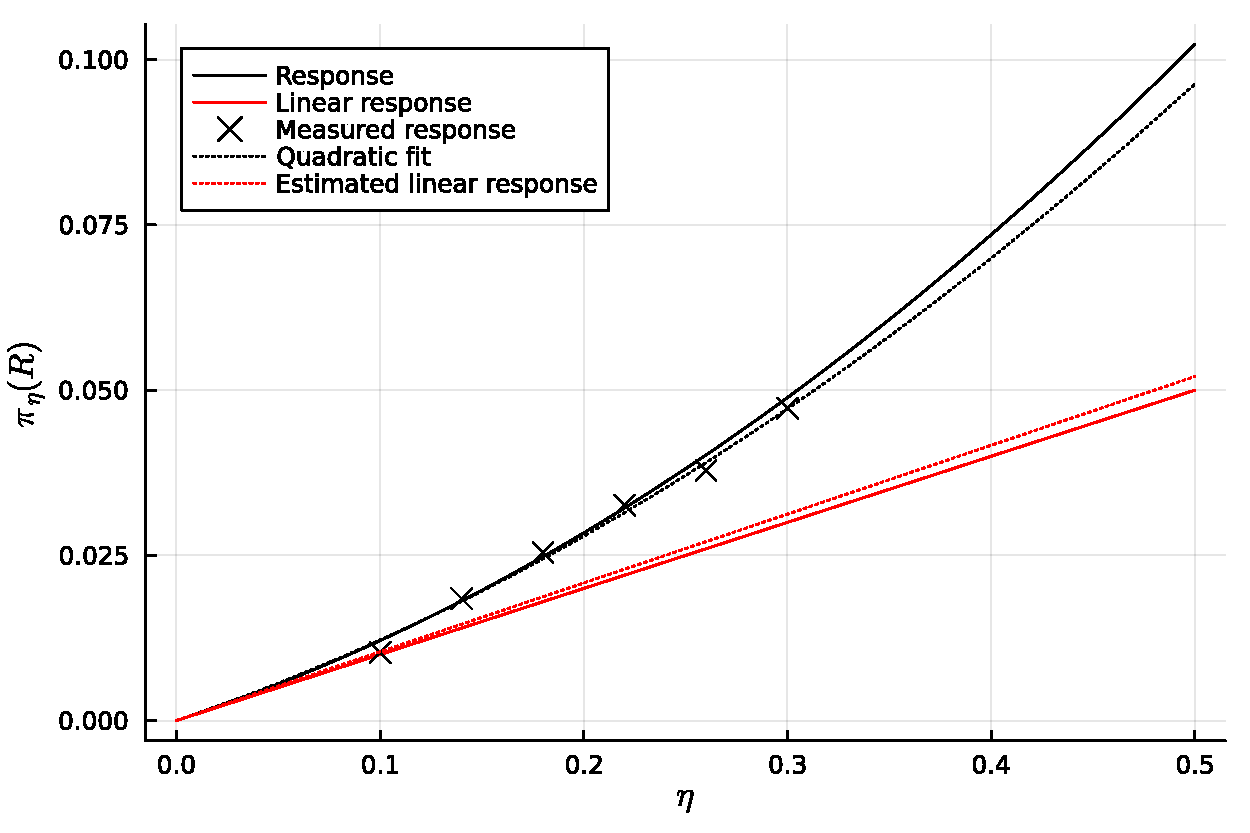
\includegraphics[width=0.7\textwidth]{figures/01/linear_response.pdf}
    \caption{Typical nonequilibrium response profile for a flux~$R$ with respect to the forcing magnitude, together with its linear response. In dotted lines, NEMD estimators of the nonlinear and linear response profiles, based on a quadratic model for sampled averages, represented by black crosses.}
    \label{fig:01:linear_response}
\end{figure}

\noe{Arguer que le coeff de transport est une quantité dynamique -> certes, il n'est défini au fond qu'en termes de nonequilibrium ensemble averages.
Mais l'ensemble est implicitement par une dynamique, et -- le seul moyen de calculer un coeff de transport est d'avoir accès à de longues trajectoires -- pas de reweighting possible par exemple. Mais l'argument "massue" est donné par la formule de Green--Kubo.
}

\paragraph{Connection with equilibrium fluctuations}
\label{subsec:linear_response_theory}
We briefly present linear response results giving alternative expressions for the coefficient~$\alpha$ in terms of equilibrium dynamical averages, and form the basis of numerical methods such as the celebrated Green--Kubo formula~\cite{G54,K57a,K57b}. Here, we only give a somewhat informal presentation in the~$L^2(\pi)$ framework, but we stress that similar results can be proven for a broad class of systems and functional settings, see for example~\cite{H10} or~\cite[Section 5.2]{LS16}.

We present two derivations of the Green--Kubo formula.
\paragraph{Expansion of the nonequilibrium steady state.}
This derivation assumes that the nonequilibrium steady-state~$\pi_\eta$ admits a probability density with respect to the equilibrium steady-state~$\pi$, which can be perturbatively expanded (for~$|\eta|$ sufficiently small) into a power series
\begin{equation}
    \label{eq:01:nemd_steady_state_expansion}
    \pi_\eta=\pi\sum_{k=0}^\infty \eta^k\psi_k,
\end{equation}
where~$\psi_k\in L^2(\pi)$ for all~$k\geq 0$.

Setting~$\eta=0$ in~\eqref{eq:01:nemd_steady_state_expansion}, it necessarily holds that~$\psi_0=\1_{\cX}$.
The formal expansion~\eqref{eq:01:nemd_steady_state_expansion} can be shown to be valid when the nonequilibrium perturbation is ``small'', e.g. when~$\wcL$ is~$\cL^Y$-bounded on~$L^2(\pi)$ and~$|\eta|$ is small enough, see for instance the proof of~\cite[Theorem 5.2]{LS16}. This is the case for perturbations of the dynamics by a non-conservative force~$F$, under tame assumptions on~$F$, see Table~\ref{tab:nemd_generator_perturbations}.

Assuming the validity of such an ansatz, the stationary Fokker--Planck equation~\eqref{eq:01:fp_nemd} writes
\begin{equation}
    \label{eq:01:fp_equation_formal}
    \left(\cL_0+\eta\wcL\right)^*\sum_{k=0}^\infty \eta^k\psi_k=0,
\end{equation}
where the adjoint is with respect to the $L^2(\pi)$ scalar products.
Matching terms in~$\eta$, it therefore holds for any~$k\geq 1$ that
\begin{equation}
    \wcL^*\psi_{k-1}=-\cL_0^*\psi_k,
\end{equation}
so that in particular~$\wcL^*\1_{\cX}=-\cL_0^*\psi_1$. 

Provided the so-called conjugate flux
\begin{align}
\label{eq:conjugate_flux}
    S=\wcL^*\1_{\cX},
\end{align} 
belongs to the space~$L_0^2(\pi)$ of~$\pi$-centered observables, we may write
\begin{equation}\label{eq:psi_1}
    \psi_1=-\left(\cL_0^{-1}\right)^*S,
\end{equation}
which in turn implies, by the definition~\eqref{eq:01:linear_response} the following expression for the transport coefficient
\begin{equation}
\label{eq:01:linear_response_eq}
    \alpha = \underset{\eta\to 0}{\lim}\,\eta^{-1}\int_{\cX}\left(\1_{\cX}-\eta(\cL_0^{-1})^*S\right)R\,\d \pi- =-\int_{\cX}S\cL_0^{-1}R\,\d\pi.
\end{equation}
Note that expression for the conjugate response~$S$ can be computed explicitly by integration by parts. The expressions of the conjugate fluxes corresponding to the perturbations given in Table~\ref{tab:nemd_generator_perturbations} are given in Table~\ref{tab:conjugate_response} below, and can easily be checked to belong to~$L_0^2(\pi)$ under tame assumptions on~$V,\delta T$ and~$F$.

The formulation~\eqref{eq:01:linear_response_eq} shows that the linear response~$\alpha$ can be expressed as the equilibrium average of the observable~$-S\cL_0^{-1}R$. Unfortunately, the various equilibrium sampling methods described in Section~\ref{sec:sampling_methods} cannot be applied outright, since they require the evaluation of the solution~$\cL_0^{-1}R$ to a high-dimensional Poisson equation.

Instead, one can reformulate~\eqref{eq:01:linear_response_eq} as a dynamical average using the expression of the inverse of~$\cL^Y$ in~\eqref{eq:generator_inverse}: we obtain the celebrated Green--Kubo formula
\begin{equation}
    \label{eq:01:green_kubo}
    \alpha = \int_{0}^\infty\E_{\pi}\left[S(x_0)R(x_t)\right]\,\d t.
\end{equation}

\begin{table}[h]
    \centering
    \begin{tabular}{|c|c|c|}
        \hline
        \backslashbox{Perturbation}{Dynamics}& Overdamped Langevin&Underdamped Langevin\\
        \hline
        Non-conservative force & $\beta F\cdot \nabla V - \nabla\cdot F$ & $\beta F\cdot M^{-1}p$\\
        \hline
        Temperature profile & $\begin{aligned}&\Delta\delta T-2\beta\nabla V\cdot \nabla\delta T\\&-\delta T\left(\beta^2|\nabla V|^2-\beta\Delta V\right)\end{aligned}$ & $\beta\gamma\delta T\left(\mathrm{Tr}\,M^{-1}-\beta\left|M^{-1}p\right|^2\right)$ \\
        \hline
    \end{tabular}
    \caption{Expressions for the conjugate response~$S$, for usual dynamics and perturbation types.}
    \label{tab:conjugate_response}
\end{table}

\paragraph{First-order expansion of the average flux.}
When the perturbation~$\widetilde\cL$ is not~$\cL_0$-bounded, the expansion~\eqref{eq:01:nemd_steady_state_expansion} is not so easy to obtain. In this case, one

The Green--Kubo formula~\eqref{eq:01:green_kubo} allows for the computation of multiple transport coefficients from equilibrium trajectories of the dynamics~\eqref{eq:formal SDE}, which is convenient from a practical point of view.

% % In Section~\ref{subsec:nemd_dynamics}, we define the nonequilibrium systems we consider in this work. In Section~\ref{subsec:linear_response_theory}, we give an overview of linear response theory. In Section~\ref{subsec:transport_coefficient_examples}, we present some typical examples of nonequilibrium systems and their associated transport coefficients.


\subsection{Accelerated MD methods}
\noe{Présenter les méthodes de Voter}

\section{Mathematical descriptions of metastability}
\label{sec:01:metastability}
As mentioned previously, metastability is characterized by a dramatic separation of timescales in the system's dynamics. %generated
Mathematical formalisms of this phenomenon aim to make this notion precise, providing quantitative tools to analyze and exploit it. %generated
These formalisms can be broadly categorized into two families: global approaches, which seek to describe the dynamics as a jump process between all the metastable states of the system, and local approaches, which focus on characterizing the dynamics within a single, predefined metastable region. %generated

\subsection{Global approaches}
Global approaches aim to understand the long-time behavior of the system as a coarse-grained Markov jump process between a set of metastable states. %generated
One of the foundational frameworks for this is the potential theory developed by Freidlin and Wentzell, which describes the mean transition times between potential wells in the small noise limit. %generated
Another powerful framework, rooted in semiclassical analysis, studies the low-lying spectrum of the Witten Laplacian, an operator unitarily equivalent to the infinitesimal generator. %generated
In this picture, the small eigenvalues of the operator correspond to the slow transition rates between metastable states, providing a direct link between the spectrum and the global dynamics. %generated
<Missing Bovier and co + early semiclassical litterature>

\subsection{Local approaches}
Local approaches, by contrast, focus on the behavior of the dynamics conditioned to remain within a single predefined domain~$\Omega$, which is assumed to represent a metastable state. %generated
The central concept in this context is the Quasi-Stationary Distribution (QSD), which is the limiting distribution of the process at long times, given that it has not yet exited~$\Omega$. %generated
The QSD represents the local equilibrium state within the metastable region. %generated
Crucially, the rate of convergence to the QSD and the mean exit time from~$\Omega$ are directly related to the spectral properties of the generator~$\mathcal{L}_\beta$ with absorbing (Dirichlet) boundary conditions imposed on~$\partial\Omega$. %generated
The principal eigenvalue~$\lambda_1(\Omega)$ corresponds to the inverse mean exit time, while the spectral gap~$\lambda_2(\Omega) - \lambda_1(\Omega)$ governs the rate of relaxation to the QSD within the domain. %generated
<Introduce the QSD in detail, with some links to the biology litterature, review some of the semiclassical litterature pertaining to these approaches>

\subsection{Other numerical methods}
<Discuss briefly related numerical methods: Koopman approaches, Markov state models, and effective dynamics>

\section{Main contributions of this thesis}
\label{sec:01:contributions}
\paragraph{On the mathematical study of metastability.}
In Chapter~\ref{02:chap:semiclassic}, we extend the mathematical theory of metastability by analyzing the spectral properties of reversible diffusions in domains whose boundaries are themselves temperature-dependent. %generated
This work generalizes celebrated results like the Eyring--Kramers formula to a new setting where the definition of a metastable state is not fixed, but can adapt to the system's thermal energy. %generated
We derive precise low-temperature asymptotics for the eigenvalues of the Dirichlet generator, which provides new insights into the sensitivity of metastable behavior with respect to the shape of the confining domain. %generated
These results are motivated by the need for a rigorous foundation for modern accelerated MD algorithms, and they provide the key theoretical tools used in the subsequent chapter. %generated

\paragraph{Accelerated MD methodology.}
Building upon the mathematical results of the previous chapter, we propose in Chapter~\ref{chap:shape_optimization} a novel and principled methodology for defining metastable states. %generated
We frame the problem as one of shape optimization: we treat the boundary of a metastable domain as a variable to be optimized in order to maximize the separation of timescales within it. %generated
Our objective function is the ratio of the spectral gap to the principal eigenvalue, a metric directly linked to the efficiency of accelerated sampling methods like Parallel Replica. %generated
We develop a robust numerical algorithm for this optimization, using analytical expressions for shape variations of Dirichlet eigenvalues to perform a local ascent in the space of possible domain shapes. %generated

\paragraph{Nonequilibrium sampling.}
In Chapter~\ref{04:chap:norton}, we shift our focus from equilibrium and metastable dynamics to the computation of transport coefficients in nonequilibrium systems. %generated
We introduce and develop a stochastic version of the Norton dynamics, which provides a dual approach to standard NEMD simulations. %generated
Instead of fixing an external force and measuring the resulting flux, this method fixes the flux and measures the average force required to sustain it. %generated
We develop the formal theory for this class of constrained diffusion processes and provide numerical evidence that this approach can be equivalent to, and in some cases more efficient than, standard NEMD methods. %generated

\paragraph{Modelling.}
Finally, in Chapter~\ref{chap:overdamped}, we address a foundational question in the modelling of molecular systems: the validity of the overdamped (Kramers--Smoluchowski) approximation. %generated
We provide a new, simple proof for the convergence of the kinetic Langevin dynamics to the overdamped limit in the case of a position-dependent, matrix-valued friction. %generated
Our approach is based on functional-analytic estimates from hypocoercivity theory, offering a more direct alternative to traditional stochastic averaging methods and providing an intuitive explanation for the emergence of the noise-induced drift term. %generated
%%%%


% \paragraph{MCMC methods.}
% The common tool unifying these methods is the Metropolis--Hastings algorithm~\cite{MRTT53}, which provides a general method for constructing reversible Markov chains with respect to a target probability measure~$\pi$ on~$\cE$ whose density is known up to a normalization constant.
% \noe{pas sur de vouloir rentrer dans trop de détails}
% The algorithm relies on the definition of a proposition mechanism, which is a Markov transition kernel defined on~$\cX$, with an explicit density~$T:\cX\times\cX\to\R_+$.
% - Various proposal schemes: Random walk Metropolis-Hastings, proposals based on numerical schemes (MALA,HMC), Generative models, Kernels in CV space


% \paragraph{Langevin dynamics and its overdamped limit.}
% We now turn to methods based on ergodic dynamics.

% The~\textit{underdamped Langevin dynamics} are defined as solutions to the following stochastic differential equation (SDE) on~$\cE$
% \begin{equation}
%     \label{eq:01:underdamped_langevin}
%     \left\{\begin{aligned}
%     \d q^\gamma_t &= M^{-1}p^\gamma_t\,\d t,\\
%     \d p^\gamma_t &= -\nabla V(q^\gamma_t)\,\d t -\gamma M^{-1}p^\gamma_t\,\d t + \sqrt{\frac{2\gamma}{\beta}}\,\d W_t,
%     \end{aligned}\right.
% \end{equation}
% where~$W$ is a~$3N$-dimensional Brownian motion, and~$\gamma>0$ is a friction parameter. The Langevin equation~\eqref{eq:01:underdamped_langevin} can been formally derived as the (Hamiltonian) dynamics of a single particle harmonically bound to a~``heat-bath'' of~$M$ coupled harmonic oscillators, in the limit~$M\to+\infty$, see~\cite{FKM65}.


% When~$\gamma=0$, the underdamped Langevin dynamics corresponds to the Hamiltonian dynamics, while in the limit~$\gamma\to 0$ it can be shown (see for example Chapter~\ref{chap:overdamped} for a precise statement and proof) that the time-rescaled trajectories
% \begin{equation}
%     \left(q^\gamma_{\gamma t},p^\gamma_{\gamma t}\right)_{0\leq t\leq T} \xrightarrow{\gamma\to 0} (X_t)_{0\leq t\leq T},
% \end{equation}
% where~$X_t$ solves the so-called~\textit{overdamped Langevin equation}, which is the SDE
% \begin{equation}
%     \label{eq:01:overdamped_langevin}
%     \d X_t = -\nabla V(X_t)\,\d t + \sqrt{\frac{2}{\beta}}\,\d W_t.
% \end{equation}
% - Highlight distinction with Monte Carlo: relies on the ergodicity of a continuous-time dynamics -- existence of a timestep bias
% - Formula for standard underdamped Langevin dynamics -- + more general diffusion and frictions coefficients
% - Historical reference of derivation from Hamiltonian dynamics of coupled oscillators (Ford, Kac, Mazur)
% - Overdamped limit -- link with MALA

% \paragraph{Discretization of the Langevin dynamics}
% - Splitting schemes

% % \paragraph{Link to optimization.} % SECONDAIRE
% % - Nesterov = Langevin
% % - SGD = Overdamped Langevin (find references for both)

% \paragraph{The generator and its spectrum.}

% % SECONDAIRE: 
% % \paragraph{Other dynamics}
% % - PDMPS
% % - Adaptive and Generalized Langevin

% % \paragraph{Variance reduction.}
% % - Importance sampling = biasing potentials
% % - Stratification = umbrella sampling
% % - Control variates = ??
% % - Symmetrization

% \subsection{The trajectorial sampling problem.}
% \label{sec:01:dynamical_properties}
% We now turn the main motivation for the problems considered in this thesis, and the second important application of MD, namely the measurement of dynamical properties. These can be understood abstractly as average properties---not of the microstate, as defined by~\eqref{eq:01:ensemble_average}--- but of the microstate trajectories themselves.
% These include:
% \begin{itemize}
%     \item{\textit{Response properties}}
%     \item{\textit{Transition statistics}}
%     \item{\textit{Path sampling}}
% \end{itemize}

% All these properties rely on the ability to sample unbiased and sufficiently long trajectories of the equilibrium dynamics (\eqref{eq:01:underdamped_langevin} or~\eqref{eq:01:overdamped_langevin}).

% \paragraph{Transport coefficient computations.}
% - Green--Kubo
% - NEMD

% \paragraph{Dynamical coarse-graining.}
- state to state dynamics

% \paragraph{Variance reduction.}
% - Importance sampling = Girsanov reweighting. limited to perturbations of the drift / weights blow up in time
% - Stratification = AMS for transition paths
% - Control variates = couplings.
% - Symmetrization

% \section{Mathematical descriptions of metastability}
% \label{sec:01:metastability}
% \subsection{Global approaches}
% Semiclassical approaches - Potential-theoretic approaches à la Bovier
% \subsection{Local approaches}
% Quasi-stationary distributions - Semiclassical approaches - Analysis of the exit time - Cutoff
% \subsection{Numerical methods}
% \paragraph{Koopman methods.}
% \paragraph{Markov State Models/KMC.}
% \paragraph{Effective dynamics.}
% \paragraph{Accelerated MD methods.}
% - Hyperdynamics
% - Parallel Replica, GenParRep, ParSplice
% - Temperature-accelerated dynamics
% - Hyper and TAD rely on Eyring--Kramers formulae -- fully justified for overdamped, usable for underdamped with energetic barriers
% - ParRep only rely on existence of a QSD (possible extensions to nonequilibrium systems, e.g.), bias can be controlled with hyperparameters.

% \section{Main contributions of this thesis}
% \label{sec:01:contributions}
% \paragraph{On the mathematical study of metastability}
% - Extension of spectral asymptotics to the case of temperature-dependent boundary
% - Harmonic approximation results
% - Extended Eyring--Kramers formula
% \paragraph{Accelerated MD methodology}
% - Shape optimization 
% \paragraph{Nonequilibrium sampling}
% - Norton
% \paragraph{Modelling}
% - Kramers--Smoluchowski limit